% Options for packages loaded elsewhere
\PassOptionsToPackage{unicode}{hyperref}
\PassOptionsToPackage{hyphens}{url}
\documentclass[
]{article}
\usepackage[margin=0.75in]{geometry}
\usepackage{xcolor}
\usepackage{amsmath,amssymb}
\usepackage{graphicx}
\usepackage{placeins} % \FloatBarrier: keep figure order vs.\ later floats
\usepackage{pgfplots}
\pgfplotsset{compat=1.18}
\usepgfplotslibrary{fillbetween}
\usetikzlibrary{calc,patterns,shapes.geometric,arrows.meta,positioning}
\setcounter{secnumdepth}{-\maxdimen} % remove section numbering
\usepackage{iftex}
\ifPDFTeX
  \usepackage[T1]{fontenc}
  \usepackage[utf8]{inputenc}
  \usepackage{textcomp} % provide euro and other symbols
\else % if luatex or xetex
  \usepackage{unicode-math} % this also loads fontspec
  \defaultfontfeatures{Scale=MatchLowercase}
  \defaultfontfeatures[\rmfamily]{Ligatures=TeX,Scale=1}
\fi
\usepackage{lmodern}
\ifPDFTeX\else
  % xetex/luatex font selection
\fi
% Use upquote if available, for straight quotes in verbatim environments
\IfFileExists{upquote.sty}{\usepackage{upquote}}{}
\IfFileExists{microtype.sty}{% use microtype if available
  \usepackage[]{microtype}
  \UseMicrotypeSet[protrusion]{basicmath} % disable protrusion for tt fonts
}{}
\makeatletter
\@ifundefined{KOMAClassName}{% if non-KOMA class
  \IfFileExists{parskip.sty}{%
    \usepackage{parskip}
  }{% else
    \setlength{\parindent}{0pt}
    \setlength{\parskip}{6pt plus 2pt minus 1pt}}
}{% if KOMA class
  \KOMAoptions{parskip=half}}
\makeatother
\usepackage{longtable,booktabs,array}
\newcounter{none} % for unnumbered tables
\usepackage{calc} % for calculating minipage widths
% Correct order of tables after \paragraph or \subparagraph
\usepackage{etoolbox}
\makeatletter
\patchcmd\longtable{\par}{\if@noskipsec\mbox{}\fi\par}{}{}
\makeatother
% Allow footnotes in longtable head/foot
\IfFileExists{footnotehyper.sty}{\usepackage{footnotehyper}}{\usepackage{footnote}}
\makesavenoteenv{longtable}
\setlength{\emergencystretch}{3em} % prevent overfull lines
\providecommand{\tightlist}{%
  \setlength{\itemsep}{0pt}\setlength{\parskip}{0pt}}
\usepackage[backend=biber,style=authortitle,maxbibnames=99,doi=false,isbn=false,url=true]{biblatex}
\addbibresource{Lead_Highways_and_Systemic_Harm.bib}
\usepackage{bookmark}
\IfFileExists{xurl.sty}{\usepackage{xurl}}{} % add URL line breaks if available
\urlstyle{same}
\hypersetup{
  hidelinks,
  pdfcreator={LaTeX via pandoc}}

\author{Emmanuel Theodore}
\date{}

\begin{document}

\section{\texorpdfstring{\textbf{The Architecture of State-Manufactured
Violence: Illicit Markets, Environmental Neurotoxicity, Spatial
Disadvantage, and Constitutional Complicity}}{The Architecture of State-Manufactured Violence: Illicit Markets, Environmental Neurotoxicity, Spatial Disadvantage, and Constitutional Complicity}}\label{the-architecture-of-state-manufactured-violence}

\subsection{\texorpdfstring{\textbf{Introduction}}{Introduction}}\label{introduction}

The American crime surge of the late twentieth century, which reached
its terrifying zenith in the early 1990s, is frequently analyzed through
a reductionist lens. Conventional historical and political narratives
often attribute the catastrophic spike in urban violence to spontaneous
moral decay, localized cultural failures, or the sudden, unpredictable
emergence of highly addictive narcotics such as crack cocaine. However,
a rigorous, interdisciplinary diagnostic reveals a far more insidious
reality: the violence of the late twentieth century was not an isolated,
organic phenomenon, nor was it primarily the result of individual
pathology. Rather, it was the mathematically predictable culmination of
overlapping, state-manufactured crises spanning several decades.
Understanding the etiology of American urban violence requires mapping
the volatile intersections of legislative prohibition, corporate
malfeasance, environmental neurotoxicity, and racially targeted spatial
engineering.\\
To fully deconstruct how these elements are inextricably intertwined,
one must examine the mechanisms through which the state fundamentally
engineers violent ecosystems. By drawing structural parallels between
the violence of the 1920s Alcohol Prohibition era and the 1980s and
1990s War on Drugs, it becomes evident that the state routinely births
violent black markets through the criminalization of inelastic public
demand. Furthermore, the sheer biological severity and spatial
concentration of the late-century crime epidemic were profoundly
exacerbated by the ubiquitous distribution of a known
neurotoxin---tetraethyllead (TEL)---in automotive fuel. The introduction
of TEL was championed by the automotive and petroleum industries, who
systematically suppressed evidence of its lethal psychiatric and
behavioral effects for decades with the tacit complicity of the federal
government.\\
Finally, the deployment of the Federal-Aid Highway Act of 1956 operated
as an instrument of spatial weaponization, intentionally routing massive
infrastructure through redlined Black communities. While an explicit
documentary intent to poison these specific populations with aerosolized
lead exhaust may lack a single ``smoking gun'' memo, the intent to
dismantle these communities through ``slum clearance'' and
segregationist planning was explicitly codified. The resulting
neurotoxic bombardment of marginalized populations was therefore a
devastating, foreseeable, and accepted byproduct of systemic racism.
Moreover, aerosolized lead from highways was only one delivery vector.
Millions of lead service lines in residential plumbing and untested,
unremediated lead fixtures in underfunded schools constituted parallel
exposure pathways---all concentrated in the same redlined neighborhoods
by the property-tax funding architecture that sorts infrastructure
quality by race and wealth.\\
This exhaustive report synthesizes these historical, biological, and
sociological frameworks to demonstrate exactly how the state
manufactured the conditions for unprecedented urban violence, suppressed
the biological realities of that violence, and ultimately weaponized the
resulting crisis to exponentially expand its carceral and regulatory
apparatus. It further demonstrates that the legal standard ostensibly
designed to detect racial discrimination---the ``discriminatory intent''
requirement of the Fourteenth Amendment---functions not as a diagnostic
tool but as a component of the concealment apparatus, immunizing
precisely the sophisticated, coded forms of racial targeting that
political operatives have openly admitted to deploying. Finally, it
deconstructs the Fourteenth Amendment jurisprudence that continues to
shield systemic environmental racism from constitutional scrutiny,
rendering the judiciary constitutionally blind to the very
infrastructure of oppression it was designed to remedy.

\subsection{\texorpdfstring{\textbf{The Structural Mechanics of Illicit
Markets: Parallels Between the 1920s and
1990s}}{The Structural Mechanics of Illicit Markets: Parallels Between the 1920s and 1990s}}\label{the-structural-mechanics-of-illicit-markets-parallels-between-the-1920s-and-1990s}

To comprehend the explosive violence of the 1990s, an analysis must
first examine the legislative blueprint established during the 1920s. In
both eras, the federal government enacted strict prohibitionary policies
targeting substances that were either deeply ingrained in American
culture or highly demanded by specific socioeconomic populations. The
Volstead Act of 1920 and the Anti-Drug Abuse Act of 1986 operated on
identical criminogenic mechanics: neither policy eliminated public
demand; rather, they instantaneously transferred the entirety of the
supply chain and its massive revenue streams from the regulated economy
into the criminal underworld.

\subsubsection{\texorpdfstring{\textbf{The Mandatory Nature of
Competitive
Violence}}{The Mandatory Nature of Competitive Violence}}\label{the-mandatory-nature-of-competitive-violence}

When illicit markets are legislatively engineered, the participants
within those markets are fundamentally excluded from the state's legal
mechanisms for dispute resolution. A bootlegger operating in 1925 or a
crack cocaine distributor operating in 1990 could not sue a supplier for
breach of contract, seek arbitration for territorial disputes, or rely
on municipal law enforcement for protection against theft or extortion.
Consequently, violence became the mandatory, structural mechanism for
enforcing contracts, maintaining territorial monopolies, and regulating
the underground economy. The extreme violence witnessed during these
eras was not necessarily the result of psychopharmacological
intoxication---meaning it was not caused by users becoming inebriated
and spontaneously violent---but was instead the byproduct of intense,
competitive market violence between rival factions fighting for control
of lucrative distribution networks.\\
During the 1920s, the localized, decentralized street gangs of American
cities were forced to undergo a rapid, corporate evolution. The
logistical demands of importing, brewing, and distributing illegal
alcohol required a level of organization that transcended traditional
street crime. Syndicates formed, and figures like Al Capone in Chicago
and Filippo Buccola in New England utilized lethal force to consolidate
power, absorb rivals, and establish regional cartels. Decades later, the
introduction of crack cocaine into economically hollowed-out,
deindustrialized urban centers provided a similar, massive market
catalyst. In the absence of legitimate employment opportunities, the
lucrative retail model of crack cocaine transformed neighborhood youth
gangs into highly armed, entrepreneurial drug-trafficking organizations
that utilized lethal violence for territorial defense and market share
expansion.

\subsubsection{\texorpdfstring{\textbf{Empirical Trajectories of Lethal
Violence}}{Empirical Trajectories of Lethal Violence}}\label{empirical-trajectories-of-lethal-violence}

The statistical topography of lethal violence in both eras reveals
striking, undeniable parallels. In both instances, the enactment of
prohibitionary policies caused the national homicide rate to effectively
double from its pre-prohibition baseline, reaching historic apexes
before collapsing only when the underlying market dynamics shifted.

{\def\LTcaptype{none} % do not increment counter
\begin{longtable}[]{@{}
  >{\raggedright\arraybackslash}p{(\linewidth - 4\tabcolsep) * \real{0.3333}}
  >{\raggedright\arraybackslash}p{(\linewidth - 4\tabcolsep) * \real{0.3333}}
  >{\raggedright\arraybackslash}p{(\linewidth - 4\tabcolsep) * \real{0.3333}}@{}}
\toprule\noalign{}
\begin{minipage}[b]{\linewidth}\raggedright
Metric / Era
\end{minipage} & \begin{minipage}[b]{\linewidth}\raggedright
1920s Prohibition Era
\end{minipage} & \begin{minipage}[b]{\linewidth}\raggedright
1980s-1990s Crack Epidemic
\end{minipage} \\
\midrule\noalign{}
\endhead
\bottomrule\noalign{}
\endlastfoot
\textbf{Pre-Crisis Baseline Homicide Rate} & \textasciitilde4.6 to 5.9
per 100,000 (1910-1915) & 5.1 per 100,000 (1960) \\
\textbf{Peak Homicide Rate} & \textasciitilde9.8 to 10.0 per 100,000
(1933) & 9.8 to 10.2 per 100,000 (1980, 1991) \\
\textbf{Catalyst Commodity} & Illicit Alcohol (Hard Liquor) & Crack
Cocaine \\
\textbf{Primary Force Multiplier} & Thompson Submachine Gun &
High-Capacity Concealable Handguns \\
\textbf{Market Correction / Violence Decline} & Repeal of the 18th
Amendment (1933) & Natural abatement of crack markets (late 1990s) \\
\end{longtable}
}

\emph{Data synthesized from historical U.S. Vital Statistics, Bureau of
the Census reconstructions, and FBI Uniform Crime Reports.}

\begin{figure}[ht]
\centering
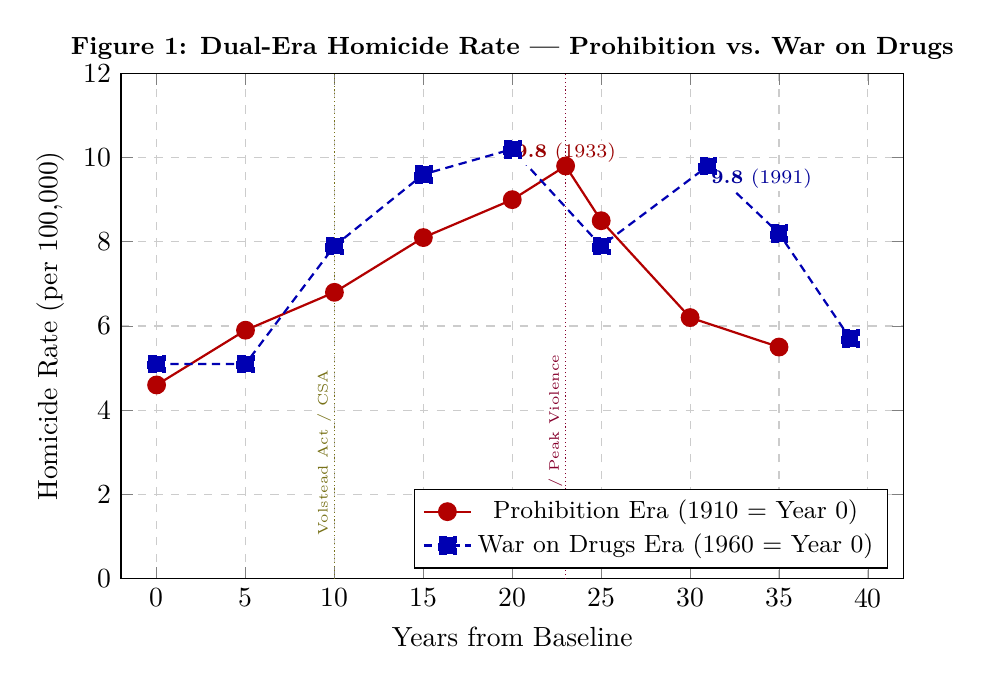
\begin{tikzpicture}
\begin{axis}[
    width=0.95\textwidth,
    height=8cm,
    title={\textbf{Figure 1: Dual-Era Homicide Rate --- Prohibition vs.\ War on Drugs}},
    xlabel={Years from Baseline},
    ylabel={Homicide Rate (per 100{,}000)},
    xmin=-2, xmax=42,
    ymin=0, ymax=12,
    xtick={0,5,10,15,20,25,30,35,40},
    ytick={0,2,4,6,8,10,12},
    grid=major,
    grid style={dashed, gray!40},
    mark size=3pt,
    every axis title/.style={font=\bfseries\small, at={(0.5,1.05)}},
    legend style={at={(0.98,0.02)}, anchor=south east, font=\small},
]
% Prohibition era: baseline 1910=year 0
\addplot[thick, red!70!black, mark=*] coordinates {
    (0, 4.6) (5, 5.9) (10, 6.8) (15, 8.1) (20, 9.0) (23, 9.8) (25, 8.5) (30, 6.2) (35, 5.5)
};
\addlegendentry{Prohibition Era (1910 = Year 0)}
% War on Drugs era: baseline 1960=year 0
\addplot[thick, blue!70!black, mark=square*, densely dashed] coordinates {
    (0, 5.1) (5, 5.1) (10, 7.9) (15, 9.6) (20, 10.2) (25, 7.9) (31, 9.8) (35, 8.2) (39, 5.7)
};
\addlegendentry{War on Drugs Era (1960 = Year 0)}
% Annotations
\node[above, font=\scriptsize, red!60!black, fill=white, inner sep=1pt] at (axis cs:23,9.8) {\textbf{9.8} (1933)};
\node[below right, font=\scriptsize, blue!60!black, fill=white, inner sep=1pt] at (axis cs:31,9.8) {\textbf{9.8} (1991)};
% Policy lines
\draw[densely dotted, olive!80!black] (axis cs:10,0) -- (axis cs:10,12);
\node[rotate=90, anchor=south, font=\tiny, olive!80!black, fill=white, inner sep=1pt] at (axis cs:10,3) {Volstead Act / CSA};
\draw[densely dotted, purple!70!black] (axis cs:23,0) -- (axis cs:23,12);
\node[rotate=90, anchor=south, font=\tiny, purple!70!black, fill=white, inner sep=1pt] at (axis cs:23,3) {Repeal / Peak Violence};
\end{axis}
\end{tikzpicture}
\caption*{\parbox{\linewidth}{\raggedright\small\emph{Sources: U.S.\ Vital Statistics; Bureau of the Census historical reconstructions; FBI UCR. Both eras are aligned at their respective pre-prohibition baselines (1910 and 1960). Both trajectories peak at approximately 9.8 homicides per 100{,}000---the identical lethal zenith---before declining only when the underlying market dynamics shifted (repeal of Prohibition; natural waning of crack markets).}}}
\end{figure}

\subsubsection{\texorpdfstring{\textbf{The Iron Law of Prohibition and
Toxic
Escalation}}{The Iron Law of Prohibition and Toxic Escalation}}\label{the-iron-law-of-prohibition-and-toxic-escalation}

Both eras vividly demonstrate the ``Iron Law of Prohibition,'' an
economic and pharmacological principle dictating that as law enforcement
pressure against an illicit substance increases, the potency, toxicity,
and lethality of that substance will inevitably rise. Because criminal
enterprises operate under the constant threat of detection and seizure,
bulky or low-potency products become economically unviable to smuggle,
store, or manufacture.\\
In the 1920s, the market organically shifted away from bulky beer and
wine toward highly concentrated hard liquors to maximize the
profit-to-volume ratio. To further maximize profit margins, bootleggers
frequently adulterated pure alcohol with dangerous chemical additives.
When criminal chemists attempted to re-distill industrial
alcohol---which the federal government had intentionally poisoned with
denaturing additives to deter human consumption---the results were
catastrophic. More insidiously, when the federal government intentionally poisoned
industrial alcohol with denaturing additives to prevent human
consumption, criminal chemists attempted to re-distill the liquid. The
results were catastrophic; tainted liquors containing carbolic acid or
pure wood alcohol (nicknamed ``Smoke'') caused mass casualties, killing,
blinding, or paralyzing tens of thousands of Americans during the
Prohibition era.\\
The immense logistical demands of these illicit markets fundamentally
altered the structure of organized crime. Prior to 1920, urban criminal
gangs existed on the periphery of society, engaging in fractured,
localized extortion and burglary. Prohibition provided these disparate
groups with an astronomical economic engine. Bootlegging required
purchasing defunct breweries, acquiring fleets of armored trucks and
speedboats, managing complex international supply chains---such as the
famous offshore ``Rum Row''---and laundering millions of dollars.
Criminals were forced to evolve into corporate executives, employing
lawyers, accountants, and heavily armed enforcers. Visionary mobsters
like Charles ``Lucky'' Luciano reorganized the fractured New York
underworld into the highly structured ``Five Families'' and established
``The Commission'' to mediate disputes across ethnic lines. In Chicago,
Al Capone's Outfit generated an estimated \$100 million in annual
revenue by the late 1920s, securing his empire by distributing \$500,000
monthly to bribe police officers, judges, and politicians.\\
In the 1980s, the market underwent a similar organic shift, moving from
bulky, expensive powder cocaine to highly concentrated, inexpensive, and
intensely addictive crack cocaine. This retail model allowed for
single-dose increments that flooded marginalized neighborhoods,
triggering localized public health catastrophes and unprecedented
addiction rates in the urban core.

\begin{figure}[ht]
\centering
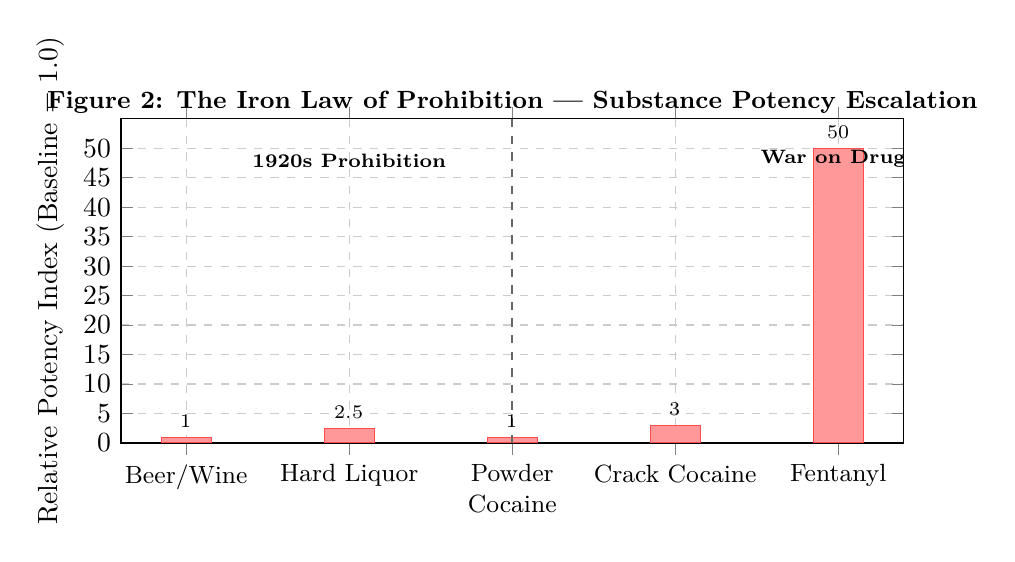
\begin{tikzpicture}
\begin{axis}[
    width=0.95\textwidth,
    height=5.7cm,
    title={\textbf{Figure 2: The Iron Law of Prohibition --- Substance Potency Escalation}},
    ybar,
    bar width=18pt,
    ylabel={Relative Potency Index (Baseline = 1.0)},
    symbolic x coords={Beer/Wine,Hard Liquor,Powder Cocaine,Crack Cocaine,Fentanyl},
    xtick=data,
    xticklabel style={font=\small, text width=2.2cm, align=center},
    ymin=0, ymax=55,
    ytick={0,5,10,15,20,25,30,35,40,45,50},
    grid=major,
    grid style={dashed, gray!40},
    every axis title/.style={font=\bfseries\small, at={(0.5,1.05)}},
    nodes near coords,
    nodes near coords style={font=\scriptsize\bfseries},
]
\addplot[fill=red!40, draw=red!70] coordinates {
    (Beer/Wine,1.0) (Hard Liquor,2.5) (Powder Cocaine,1.0) (Crack Cocaine,3.0) (Fentanyl,50.0)
};
\draw[thick, dashed, black!60] (axis cs:Powder Cocaine,0) -- (axis cs:Powder Cocaine,55);
\node[font=\scriptsize, anchor=south] at (axis cs:Hard Liquor,45) {\textbf{1920s Prohibition}};
\node[font=\scriptsize, anchor=south] at (axis cs:Fentanyl,45) {\textbf{War on Drugs}};
\end{axis}
\end{tikzpicture}
\caption*{\parbox{\linewidth}{\raggedright\small\emph{Sources: Mark Thornton, ``The Economics of Prohibition'' (1991); DEA National Drug Threat Assessment (annual); pharmacological literature. The Iron Law dictates that enforcement pressure shifts markets toward maximum potency-to-volume ratio. Prohibition-era alcohol potency increased approximately 150\%. In the modern era, the market trajectory from powder cocaine to crack to synthetic fentanyl (50--100$\times$ the potency of morphine) represents the same pharmacological escalation under identical economic pressures.}}}
\end{figure}
\FloatBarrier

Rigorous epidemiological analyses of the Chicago Historical Homicide
Project demonstrate that during Prohibition, total homicides increased
by 21 percent, yet the rate of homicides committed by individuals under
the direct influence of alcohol remained statistically unchanged. This
proves the violence was a structural byproduct of the market rather than
a chemical byproduct of the drug. This exact pattern repeated in the
1980s, where youth homicide rates (ages 14 to 24) doubled due to
territorial disputes in the drug trade, while the homicide rate for
older demographics remained essentially flat, indicating the violence
was hyper-concentrated in the youth demographic actively participating
in the illicit street-level economy.

\subsection{\texorpdfstring{\textbf{The Weaponization of Crisis: The NFA
1934 and the 1994 Crime
Bill}}{The Weaponization of Crisis: The NFA 1934 and the 1994 Crime Bill}}\label{the-weaponization-of-crisis-the-nfa-1934-and-the-1994-crime-bill}

The ultimate parallel between the 1920s and the 1990s lies in how the
state responded to the violence it had structurally engineered. In both
eras, the state leveraged the spectacular, highly publicized violence
generated by its own prohibitionary policies to justify sweeping,
permanent expansions of federal police authority, regulatory overreach,
and the carceral apparatus. This dynamic represents a recurring,
systemic algorithm in American public policy.\\
As gangland warfare escalated in the late 1920s, public tolerance for
the bootleggers evaporated. The apex of this brutality---and the direct
catalyst for federal legislative expansion---was the St.~Valentine's Day
Massacre on February 14, 1929. Associates of Al Capone's Outfit executed
seven members of George ``Bugs'' Moran's North Side Gang in a Chicago
garage, utilizing two Thompson submachine guns and two shotguns to
unleash a devastating barrage of 70 rounds. The sheer barbarity of this
event acted as a profound psychological interface shift for the American
electorate. Seizing the political capital generated by this terror, the
administration of President Franklin D. Roosevelt declared a national
``War on Crime''.\\
Attorney General Homer S. Cummings, recognizing that the federal
government lacked the constitutional authority to outright ban firearms
under the prevailing interpretations of the Second Amendment and the
Interstate Commerce Clause, drafted the National Firearms Act (NFA) of
1934. The legislative strategy ingeniously utilized Congress's
enumerated Article I power to levy taxes. The NFA mandated the
registration of specific ``gangster weapons''---defined as machine guns,
short-barreled rifles, short-barreled shotguns, and suppressors
(silencers)---and imposed a staggering \$200 transfer and making tax. In
1934, this tax (equivalent to roughly \$3,600 in modern currency)
effectively doubled or tripled the cost of the weapon. The underlying
purpose of the NFA was explicitly not revenue collection, but absolute
prohibition via prohibitive pricing and strict registration
requirements. Cummings explicitly admitted this legislative
sleight-of-hand during committee hearings, acknowledging that while a
ban might be unconstitutional, a prohibitive tax was within the law.
This maneuver provided the fledgling FBI and Treasury agents with a
powerful legal mechanism to arrest and imprison cartel members for tax
evasion or possession of unregistered firearms when underlying charges
of murder or extortion could not be proven. The NFA set a profound legal
precedent that the federal government would subsequently utilize to
draft the Marihuana Tax Act of 1937, officially launching the federal
war on drugs using the exact same constitutional mechanism of
prohibitive taxation.\\
Sixty years later, politicians faced profound public anxiety over the
crack epidemic, the proliferation of concealable handguns, and soaring
homicide rates. Following the exact legislative playbook of the 1930s,
the state expanded its punitive reach. The Violent Crime Control and Law
Enforcement Act of 1994, authored primarily by Senator Joe Biden and
championed by President Bill Clinton, became the most sweeping crime
legislation in U.S. history. The bill authorized \$9 billion for prison
construction, funded the hiring of 100,000 new police officers, expanded
the federal death penalty, and instituted harsh ``three-strikes''
mandatory life sentences.\\
Rather than addressing the systemic economic voids left by
deindustrialization, the state relied upon a carceral apparatus rooted
in post-Civil War subjugation to warehouse millions of predominantly
Black and Hispanic men. In both 1934 and 1994, the state presented an
asymmetric choice: terrorized minority communities, desperate to staunch
the bleeding in their neighborhoods, were offered punitive state
intervention in the form of mass policing and incarceration, while their
desperate requests for holistic, economic investments, drug treatment,
and community infrastructure were mocked as ``pork'' and entirely
denied.

\begin{figure}[htbp]
\centering
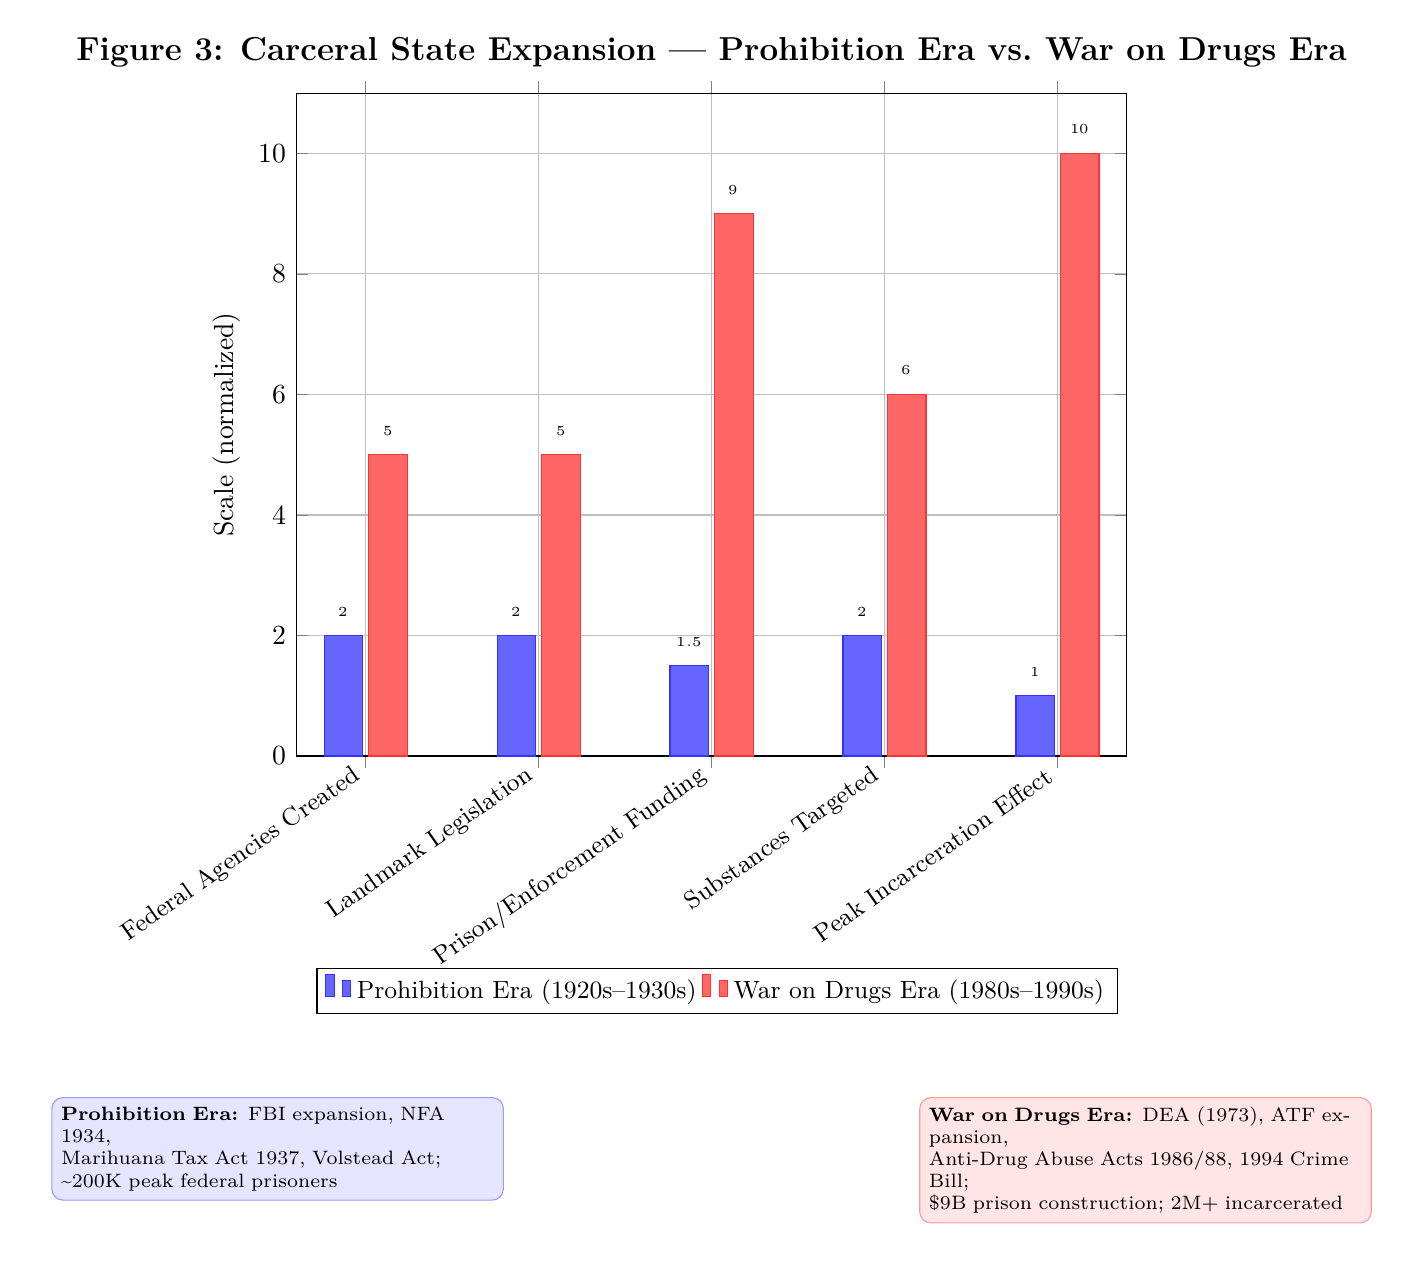
\begin{tikzpicture}
\begin{axis}[
    ybar,
    bar width=14pt,
    width=\textwidth,
    height=10cm,
    clip=false,
    ylabel={Scale (normalized)},
    symbolic x coords={Federal Agencies Created,Landmark Legislation,Prison/Enforcement Funding,Substances Targeted,Peak Incarceration Effect},
    xtick=data,
    x tick label style={rotate=35, anchor=east, font=\small},
    ymin=0, ymax=11,
    legend style={at={(0.99,-0.32)}, anchor=north east, legend columns=2, font=\small},
    nodes near coords,
    every node near coord/.append style={font=\tiny, yshift=0.12cm},
    grid=major,
    title={\textbf{Figure 3: Carceral State Expansion --- Prohibition Era vs.\ War on Drugs Era}},
    title style={font=\large},
]
% Prohibition Era (1920s-1930s)
\addplot[fill=blue!60, draw=blue!80] coordinates {
(Federal Agencies Created,2)
(Landmark Legislation,2)
(Prison/Enforcement Funding,1.5)
(Substances Targeted,2)
(Peak Incarceration Effect,1)
};
% War on Drugs Era (1980s-1990s)
\addplot[fill=red!60, draw=red!80] coordinates {
(Federal Agencies Created,5)
(Landmark Legislation,5)
(Prison/Enforcement Funding,9)
(Substances Targeted,6)
(Peak Incarceration Effect,10)
};
\legend{Prohibition Era (1920s--1930s), War on Drugs Era (1980s--1990s)}
\end{axis}

% Annotation boxes (below legend; extra yshift + bbox pad avoids PDF clipping)
\node[anchor=north west, font=\scriptsize, text width=5.5cm, fill=blue!10, draw=blue!40, rounded corners] at ([xshift=-0.2cm, yshift=-1.05cm]current axis.outer south west) {
\textbf{Prohibition Era:} FBI expansion, NFA 1934,\\
Marihuana Tax Act 1937, Volstead Act;\\
\textasciitilde 200K peak federal prisoners
};
\node[anchor=north east, font=\scriptsize, text width=5.5cm, fill=red!10, draw=red!40, rounded corners] at ([xshift=0.2cm, yshift=-1.05cm]current axis.outer south east) {
\textbf{War on Drugs Era:} DEA (1973), ATF expansion,\\
Anti-Drug Abuse Acts 1986/88, 1994 Crime Bill;\\
\$9B prison construction; 2M+ incarcerated
};
\path ([xshift=-0.5cm,yshift=-2.85cm]current axis.outer south west)
      ([xshift=0.5cm,yshift=-2.85cm]current axis.outer south east);
\end{tikzpicture}
\caption*{\emph{Comparative scale of carceral state expansion across the two major prohibition eras. The War on Drugs apparatus exceeded its Prohibition-era predecessor by an order of magnitude in funding, institutional growth, and incarceration impact. Normalized scale: 1 = Prohibition-era baseline, 10 = War on Drugs peak. Sources: Bureau of Justice Statistics; DOJ budget records; Mauer (2006); Alexander (2010).}}
\label{fig:carceral-expansion}
\end{figure}

\subsection{\texorpdfstring{\textbf{The Conspiracy of Lead: Big Oil's
Knowledge and the Cover-Up of
Neurotoxicity}}{The Conspiracy of Lead: Big Oil's Knowledge and the Cover-Up of Neurotoxicity}}\label{the-conspiracy-of-lead-big-oils-knowledge-and-the-cover-up-of-neurotoxicity}

While the economic mechanics of illicit markets explain the structural
environment of urban violence, and sociological theories like social
disorganization explain the behavioral context, they fundamentally fail
to account for the sheer biological magnitude and the underlying
psychological susceptibility of the populations involved in the late
twentieth century. This vast analytical gap is filled by environmental
epidemiology, specifically the mass poisoning of the American public by
tetraethyllead (TEL), a highly toxic gasoline additive. A rigorous
historical examination reveals that the petroleum and automotive
industries knew of TEL's devastating behavioral and violent effects from
its inception in the 1920s, yet engaged in a half-century conspiracy to
suppress this reality.

\subsubsection{\texorpdfstring{\textbf{The Invention of a Profitable
Poison}}{The Invention of a Profitable Poison}}\label{the-invention-of-a-profitable-poison}

In 1921, Thomas Midgley Jr.~and Charles Kettering, researchers at the
General Motors (GM) Research Corporation, were tasked with finding a
solution to engine ``knock''---a destructive, premature detonation of
fuel in early internal combustion engines that limited horsepower and
efficiency. After testing thousands of compounds, they discovered on
December 9, 1921, that adding a small amount of tetraethyllead to
gasoline allowed for higher compression, increased horsepower, and
eliminated engine knock.\\
Crucially, the decision to utilize TEL was not born of scientific
necessity, but of corporate monopolization and profit generation. It was
widely known to chemical engineers in the early 1920s that ethanol was
an incredibly effective, clean, and safe anti-knock agent. Midgley
himself had previously filed patents for alcohol blends, noting in an
internal memo that alcohol was the ``most direct route'' for converting
solar energy into fuel, and had even demonstrated a 30 percent
alcohol-gasoline blend at an engineering conference. However, ethanol
could not be patented by General Motors, it was already being widely
produced by independent distillers, and it would require up to 20
percent of fuel volume, which severely threatened the profit margins of
the petroleum industry. TEL, conversely, could be exclusively patented,
ensuring a highly lucrative, unassailable monopoly. Consequently, in
1924, General Motors and Standard Oil of New Jersey partnered to create
the Ethyl Gasoline Corporation to market and produce the lethal
additive.

\subsubsection{\texorpdfstring{\textbf{The ``Loony Gas'' Disasters and
Immediate Warnings of
Violence}}{The ``Loony Gas'' Disasters and Immediate Warnings of Violence}}\label{the-loony-gas-disasters-and-immediate-warnings-of-violence}

The toxicity of lead had been documented since antiquity; the Romans
were aware it could cause madness, and nineteenth-century physicians
documented its neurological devastation. Yet the specific dangers of
concentrated TEL were immediate, horrifying, and actively suppressed by
the nascent Ethyl Corporation. In 1923, before the product even reached
mass market, Midgley himself suffered severe lead poisoning from his own
invention, writing that his lungs were affected and he needed a long
absence to recover in fresh air.\\
The true catastrophe, which definitively proves corporate knowledge of
TEL's psychiatric and violent effects, occurred in 1924 when mass
production commenced. At a Standard Oil refinery in Bayway, New Jersey,
workers manufacturing TEL began experiencing severe, acute lead
poisoning. Because TEL is highly lipophilic, it rapidly crosses the
blood-brain barrier, resulting in profound neurological disruption. The
facility was mockingly dubbed the ``Loony Gas building'' by employees
due to the bizarre behavior of the workers. In October 1924, the
situation escalated into a highly public disaster. Workers exhibited
horrific psychiatric symptoms: severe tremors, visual hallucinations
(such as seeing insects wriggling over their skin or wallpaper turning
into swarms of flies), paranoia, and most notably, violent, maniacal
fury that required them to be wrestled into straitjackets. Five workers
died in quick succession after wrenching fits of violent insanity, and
35 others suffered severe neurological damage. Similar deaths and
outbreaks of madness occurred at DuPont facilities in Dayton, Ohio, and
Deepwater, New Jersey, where hallucinating workers morbidly referred to
the plant as the ``House of Butterflies''.\\
The scientific community attempted to intervene immediately, proving
that the knowledge of lead's behavioral effects was available long
before the 1990s crime wave. In 1922, chemist William Mansfield Clark
wrote to the U.S. Public Health Service (PHS) warning of a ``serious
menace to public health,'' fearing that heavy lead oxide dust from
automotive exhaust would settle in the lower stratum of city streets
where citizens lived and breathed. More pointedly, Dr.~Alice Hamilton, a
pioneering Harvard physician and the nation's foremost expert in
industrial hygiene, recognized TEL as a profound threat to the populace.
Based on her experience, she publicly warned that the additive would
poison the public with slow, cumulative effects resulting in ``insomnia,
excitement, twitching muscles, hallucinations like those of delirium
tremens, even maniacal attacks and convulsions, and death''. Hamilton
presciently noted that the absence of immediate, acute deaths on the
street was no proof of safety, as chronic lead poisoning is insidious
and cumulative.

\subsubsection{\texorpdfstring{\textbf{Robert Kehoe and the Paradigm of
Manufactured
Doubt}}{Robert Kehoe and the Paradigm of Manufactured Doubt}}\label{robert-kehoe-and-the-paradigm-of-manufactured-doubt}

Following the highly publicized, violent refinery deaths in New Jersey,
the Surgeon General temporarily suspended TEL sales in May 1925 and
convened a national conference of public health experts to assess the
danger. At this critical historical juncture, the trajectory of global
environmental health was hijacked by corporate interests. Industry
representatives, such as Frank Howard, the first President of the Ethyl
Corporation, aggressively lobbied against a ban. Howard audaciously
framed TEL as a ``Gift of God'' necessary for the industrial and
automotive progress of the nation, arguing that minor occupational
hazards could not be allowed to impede civilization's advancement.\\
To control the scientific narrative and permanently neutralize public
health critics, the industry empowered Dr.~Robert A. Kehoe, a young
toxicologist who served as the medical director of the Ethyl Corporation
and the head of the industry-funded Kettering Laboratory at the
University of Cincinnati. From the 1920s through the 1960s, Kehoe served
as the primary, undisputed scientific authority on lead exposure,
deliberately establishing a paradigm of ``cascading uncertainty''. Kehoe
formulated a highly skewed, defensive evidentiary rule: the industry did
not have to prove that aerosolized TEL was safe; rather, public health
officials had to produce indisputable, overwhelming epidemiological
proof that ambient lead exhaust was actively harming the general
population before any regulations could be imposed.\\
Kehoe's research---funded entirely by General Motors, DuPont, and
Standard Oil---falsely claimed that a certain baseline level of lead in
the human body was ``normal'' and natural, and that environmental lead
from exhaust posed no cumulative danger to the public. Whenever
independent researchers or physicians raised concerns about the
behavioral effects of subclinical lead poisoning, Kehoe and the Ethyl
Corporation mobilized to discredit them, demanding absolute proof while
controlling the funding and the data. Through this relentless campaign
of manufactured doubt and corporate hegemony over scientific literature,
Kehoe successfully stalled federal regulation for half a century,
providing the pseudo-scientific cover necessary for the unchecked
emission of millions of tons of aerosolized lead into the American
environment.

\subsection{\texorpdfstring{\textbf{Government Complicity and the
Decades of
Stalling}}{Government Complicity and the Decades of Stalling}}\label{government-complicity-and-the-decades-of-stalling}

The question of whether the government knew that leaded gasoline would
produce these effects, and whether they allowed the companies to stall
for time, is answered by the historical record with a definitive
affirmative. The federal government was explicitly warned by the world's
leading toxicologists in 1925, yet chose to abdicate its regulatory
responsibility in favor of corporate expansion.\\
Following the 1925 Surgeon General's conference, the government
appointed a committee to investigate the health effects of leaded
gasoline. The committee's study, completed within months, concluded that
``insufficient evidence'' existed to ban TEL outright, effectively
adopting the Kehoe paradigm that lack of immediate evidence of mass
fatalities equated to proof of safety. In 1927, the Surgeon General set
a completely voluntary, toothless standard for the oil industry of 3
cubic centimeters of TEL per gallon, which merely reflected the maximum
amount the industry was already using, imposing zero real restraint.\\
For the next 50 years, the federal government permitted the Ethyl
Corporation and the lead industry to entirely police themselves. The
depth of the government's complicity is highlighted by the fact that in
1958, the Surgeon General actually \emph{raised} the voluntary lead
standard to 4.23 grams per gallon, falsely concluding that despite the
massive expansion of TEL use following World War II, there was no sign
the average American had sustained any measurable increase in blood lead
concentrations. This conclusion was based entirely on the flawed,
industry-funded data produced by Robert Kehoe.\\
It was not until independent, uncompromised researchers entered the
field that the government's stance was forced to change. In the 1960s,
Caltech geochemist Clair Patterson definitively proved that modern human
lead burdens were not ``normal,'' but were the result of massive, modern
industrial contamination. By analyzing pre-Columbian human bones and
ancient ice cores, Patterson demonstrated that human activity had
increased ambient lead levels by a factor of 2,000 above pre-industrial
baselines, entirely due to anthropogenic emissions like TEL. Despite facing intense persecution and defunding
efforts orchestrated by the Ethyl Corporation and the American Petroleum
Institute, Patterson's research laid the undeniable groundwork for
environmental reform. In the 1970s, pediatrician Dr.~Herbert Needleman
further dismantled the industry's narrative by demonstrating that even
low, subclinical levels of lead exposure in children were directly
correlated with decreased IQ, shortened attention spans, and disruptive
behavior. Needleman faced identical corporate harassment, with the lead
industry attempting to vilify him and destroy his academic integrity to
protect their profits.\\
Finally, armed with this independent data and empowered by the 1970
Clean Air Act, the newly formed Environmental Protection Agency (EPA)
moved against the industry. In January 1971, EPA Administrator William
D. Ruckelshaus declared that the accumulation of lead particles posed a
severe threat to public health. In December 1973, the EPA issued its
first regulations calling for a gradual, mandatory reduction of lead
content in gasoline. Naturally, the Ethyl Corporation, DuPont, and other
chemical giants immediately sued the EPA to stall the regulations
further, forcing a protracted legal battle that reached the Supreme
Court, which ultimately upheld the EPA's authority to regulate the
neurotoxin. The final ban on leaded gasoline for motor vehicles was not
fully realized in the United States until 1996---more than 70 years
after the deaths at the ``Loony Gas'' building and Alice Hamilton's dire
warnings.

\begin{figure}[ht]
\centering
\textbf{Figure 4: The Chronology of Tetraethyllead Obfuscation (1921--1996)}\\[0.35em]
% Full-width stack (avoids empty margin beside a short side caption); tight bbox --- no oversized \path
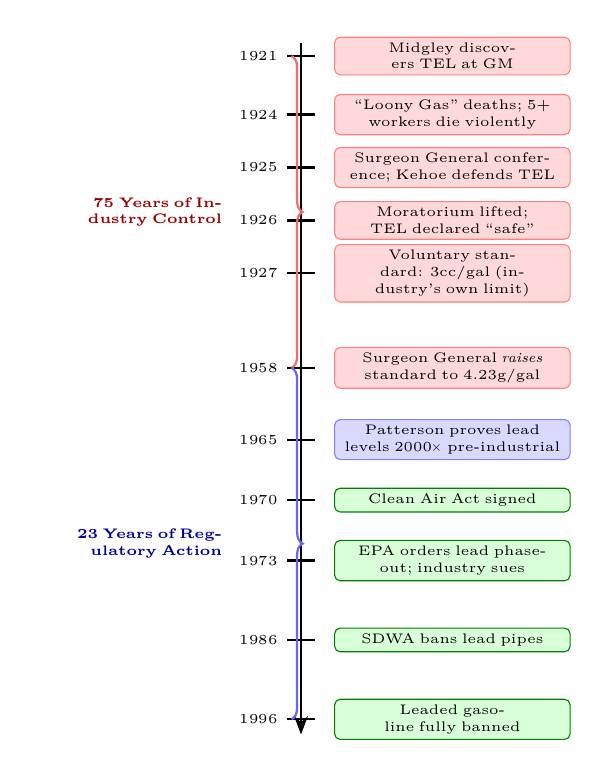
\begin{tikzpicture}[
    y=0.48cm,
    event/.style={fill=white, draw=black!50, rounded corners=2pt, font=\tiny, text width=2.85cm, align=center, inner sep=2pt},
    industry/.style={event, fill=red!15, draw=red!50},
    science/.style={event, fill=blue!15, draw=blue!50},
    policy/.style={event, fill=green!15, draw=green!50!black},
]
\pgfmathsetmacro{\ytop}{11.35}
\pgfmathsetmacro{\ybot}{-6.95}
\draw[thick, -Stealth] (0,\ytop) -- (0,\ybot);
\foreach \yr/\yy in {1921/11, 1924/9.45, 1925/8.05, 1926/6.65, 1927/5.25, 1958/2.75, 1965/0.85, 1970/-0.75, 1973/-2.35, 1986/-4.45, 1996/-6.55} {
  \draw[thick] (-0.18,\yy) -- (0.18,\yy);
  \node[left, font=\tiny\bfseries, inner sep=2pt] at (-0.22,\yy) {\pgfmathprintnumber[fixed,precision=0,set thousands separator={}]{\yr}};
}
\node[industry, anchor=west] at (0.42,11) {Midgley discovers TEL at GM};
\node[industry, anchor=west] at (0.42,9.45) {``Loony Gas'' deaths; 5+ workers die violently};
\node[industry, anchor=west] at (0.42,8.05) {Surgeon General conference; Kehoe defends TEL};
\node[industry, anchor=west] at (0.42,6.65) {Moratorium lifted; TEL declared ``safe''};
\node[industry, anchor=west] at (0.42,5.25) {Voluntary standard: 3cc/gal (industry's own limit)};
\node[industry, anchor=west] at (0.42,2.75) {Surgeon General \emph{raises} standard to 4.23g/gal};
\node[science, anchor=west] at (0.42,0.85) {Patterson proves lead levels 2000$\times$ pre-industrial};
\node[policy, anchor=west]   at (0.42,-0.75) {Clean Air Act signed};
\node[policy, anchor=west]   at (0.42,-2.35) {EPA orders lead phaseout; industry sues};
\node[policy, anchor=west]   at (0.42,-4.45) {SDWA bans lead pipes};
\node[policy, anchor=west]   at (0.42,-6.55) {Leaded gasoline fully banned};
\pgfmathsetmacro{\yFiftyEight}{2.75}
\pgfmathsetmacro{\yNinetySix}{-6.55}
\draw[thick, red!60, decorate, decoration={brace, amplitude=4pt, mirror}] (-0.12,\yFiftyEight) -- (-0.12,11);
\node[anchor=east, font=\tiny\bfseries, red!60!black, text width=2.35cm, align=right] at (-0.88,{0.5*11+0.5*\yFiftyEight}) {75 Years of Industry Control};
\draw[thick, blue!60, decorate, decoration={brace, amplitude=4pt, mirror}] (-0.12,\yNinetySix) -- (-0.12,\yFiftyEight);
\node[anchor=east, font=\tiny\bfseries, blue!60!black, text width=2.35cm, align=right] at (-0.88,{0.5*\yFiftyEight+0.5*\yNinetySix}) {23 Years of Regulatory Action};
\path (-3.2,-7.45) (3.35,11.75);
\end{tikzpicture}\\[0.45em]
\parbox{\linewidth}{\raggedright\small\emph{Red boxes indicate corporate/industry actions; blue boxes indicate independent scientific breakthroughs; green boxes indicate regulatory policy. For 75 years (1921--1996), the petroleum and automotive industries maintained near-total control over the scientific narrative on lead toxicity, utilizing the Kehoe Paradigm to shift the burden of proof from the corporation to the public. Meaningful regulation began only after Clair Patterson's independent research shattered the industry's ``normal lead levels'' mythology. Sources: Smithsonian; Columbia University; EPA historical records; Type Investigations.}}
\end{figure}

\begin{figure}[!htbp]
\centering
\textbf{Figure 5: Kehoe's ``Normal'' vs.\ Patterson's Pre-Industrial Lead Levels}\\[0.3em]
% Axis width < \textwidth: scale only axis + y tick labels + node labels otherwise spill past the margin
\begin{minipage}{\linewidth}
\centering
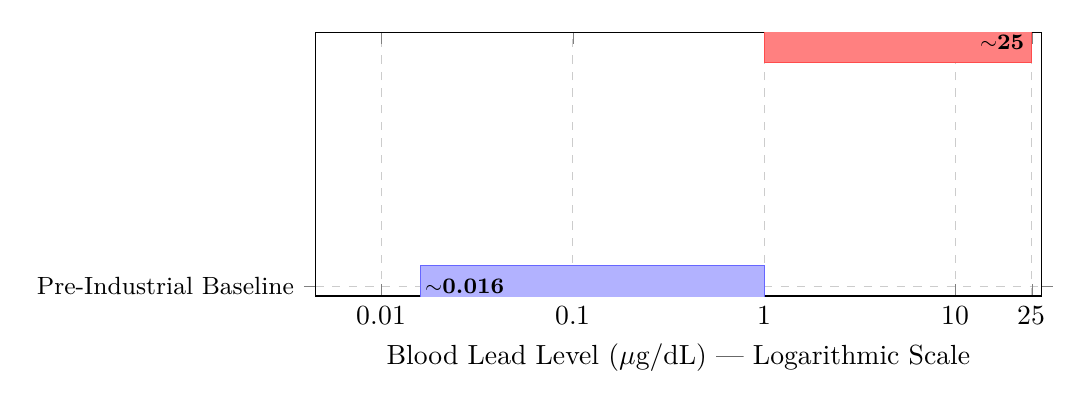
\begin{tikzpicture}
\begin{axis}[
    width=0.76\textwidth,
    height=3.35cm,
    scale only axis,
    clip=true,
    clip mode=individual,
    xbar,
    bar width=15pt,
    bar shift=0pt,
    xlabel={Blood Lead Level ($\mu$g/dL) --- Logarithmic Scale},
    symbolic y coords={Pre-Industrial Baseline,Kehoe's ``Normal''},
    ytick=data,
    yticklabel style={font=\small},
    xmin=0.01, xmax=28,
    xmode=log,
    log basis x=10,
    log ticks with fixed point,
    xtick={0.01,0.1,1,10,25},
    minor x tick num=1,
    enlarge x limits={auto=false, upper=0.04, lower=0.06},
    enlarge y limits=0.04,
    grid=major,
    grid style={dashed, gray!40},
    every axis title/.style={font=\bfseries\small, at={(0.5,1.08)}},
    point meta=explicit symbolic,
    nodes near coords={\pgfplotspointmeta},
    nodes near coords align={horizontal},
]
% Short bar: label to the right of bar tip; long bar: anchor east so $\sim$25 stays inside axis (avoids right overflow)
\addplot[fill=blue!30, draw=blue!60,
    nodes near coords style={font=\footnotesize\bfseries, anchor=west, inner sep=1.5pt},
] coordinates {(0.016,Pre-Industrial Baseline)[{$\sim$0.016}]};
\addplot[fill=red!50, draw=red!70,
    nodes near coords style={font=\footnotesize\bfseries, anchor=east, inner sep=2.5pt},
] coordinates {(25,Kehoe's ``Normal'')[{$\sim$25}]};
\end{axis}
\end{tikzpicture}
\end{minipage}\\[0.4em]
\parbox{\linewidth}{\raggedright\small\emph{Sources: Clair Patterson, ``Contaminated and Natural Lead Environments of Man,'' Archives of Environmental Health 11 (1965): 344--360; NRC, ``Measuring Lead Exposure in Infants, Children, and Other Sensitive Populations'' (1993). Patterson's analysis of pre-Columbian bones and ancient ice cores proved that Kehoe's ``normal'' blood lead level of $\sim$25 $\mu$g/dL was approximately 1{,}500$\times$ the actual pre-industrial human baseline of $\sim$0.016 $\mu$g/dL. The entire concept of ``normal'' had been manufactured by the industry.}}
\end{figure}
\FloatBarrier

\subsection{\texorpdfstring{\textbf{The Biological Vector: Lead as an
Accelerator of Aggression and
Crime}}{The Biological Vector: Lead as an Accelerator of Aggression and Crime}}\label{the-biological-vector-lead-as-an-accelerator-of-aggression-and-crime}

The consequence of the Ethyl Corporation's 50-year regulatory blockade
and the government's complicity was a mass, unconsented chemical
lobotomy of the American public. The ``lead-crime hypothesis'' posits
that the drastic, unprecedented rise in violent crime from the 1960s to
the early 1990s, and its equally sudden, unpredicted collapse, were
fundamentally driven by the rise and fall of TEL in automotive fuel.

\subsubsection{\texorpdfstring{\textbf{The Neurological Anatomy of
Violence}}{The Neurological Anatomy of Violence}}\label{the-neurological-anatomy-of-violence}

Lead is a severe, developmental neurotoxicant with no safe threshold of
exposure in the human body. When millions of tons of aerosolized lead
dust were expelled from automobile tailpipes, it settled into the soil
and dust of urban environments, where it was inevitably inhaled or
ingested by young children. Because children's bodies absorb a far
greater proportion of ingested lead than adults, and because their
central nervous systems are in critical stages of rapid development,
they are uniquely vulnerable to its devastation.\\
Once lead penetrates the blood-brain barrier, it operates as a cellular
imposter, mimicking and replacing beneficial ions such as calcium in
biological processes. Extensive biological and neuroimaging research
demonstrates that early childhood lead exposure causes permanent
architectural damage to the brain. Specifically, lead exposure reduces
regional gray matter volume in the prefrontal cortex and the anterior
cingulate cortex---the precise anatomical areas responsible for
executive function, impulse control, emotional regulation, and rational
decision-making. Simultaneously, lead alters the functioning of the
amygdala, fostering unchecked aggression, heightened impulsivity, and an
inability to regulate behavioral responses to stress.\\
The epidemiological data regarding this neurological impairment is
staggering. A comprehensive 2022 study estimated that childhood lead
exposure from automotive exhaust resulted in the loss of over 824
million IQ points among Americans alive today, and contributed to an
estimated 151 million cases of psychiatric disorders and behavioral
psychopathologies. Children exposed to lead exhibited significantly
higher rates of attention deficit hyperactivity disorder (ADHD), school
suspensions, juvenile detention, and highly aggressive, antisocial
behavior.

\subsubsection{\texorpdfstring{\textbf{The Lead-Crime
Elasticity}}{The Lead-Crime Elasticity}}\label{the-lead-crime-elasticity}

The epidemiological timeline of lead consumption aligns perfectly with
the national crime statistics when a roughly 20-year biological lag is
applied. Because the highest rates of criminal offending universally
occur in young adulthood (late teens to early twenties), the behavioral
outcomes of childhood brain poisoning predictably manifest two decades
later.

{\def\LTcaptype{none} % do not increment counter
\begin{longtable}[]{@{}
  >{\raggedright\arraybackslash}p{(\linewidth - 4\tabcolsep) * \real{0.3333}}
  >{\raggedright\arraybackslash}p{(\linewidth - 4\tabcolsep) * \real{0.3333}}
  >{\raggedright\arraybackslash}p{(\linewidth - 4\tabcolsep) * \real{0.3333}}@{}}
\toprule\noalign{}
\begin{minipage}[b]{\linewidth}\raggedright
Era
\end{minipage} & \begin{minipage}[b]{\linewidth}\raggedright
Environmental Lead Action
\end{minipage} & \begin{minipage}[b]{\linewidth}\raggedright
Societal / Criminological Result (20 Years Later)
\end{minipage} \\
\midrule\noalign{}
\endhead
\bottomrule\noalign{}
\endlastfoot
\textbf{1940s - 1970s} & Exponential rise in leaded gasoline consumption
during post-WWII auto boom. Millions of tons of TEL aerosolized into
urban air and soil. & \textbf{1960s - 1990s:} Exponential rise in
national violent crime rates. The poisoned cohort reaches young
adulthood lacking impulse control, fueling the urban crime epidemics. \\
\textbf{Late 1970s - 1980s} & EPA mandates phasedown of lead in gasoline
under the Clean Air Act. Blood-lead levels in children drop
precipitously. & \textbf{Late 1990s - 2010s:} The ``Great Crime
Decline.'' The detoxified cohort reaches young adulthood with intact
prefrontal cortices, resulting in historic drops in violent crime. \\
\end{longtable}
}

\emph{Timeline illustrating the 20-year biological lag of the lead-crime
hypothesis.}\\
Economist Jessica Wolpaw Reyes utilized the staggered phase-out of
leaded gasoline across different states as a natural experiment to
isolate this variable. Controlling for exogenous factors such as
economic conditions and policing, Reyes demonstrated a remarkably high
elasticity of 0.8 between childhood lead exposure and subsequent violent
crime. This signifies that for every 10 percent increase in lead
exposure, there was an 8 percent increase in violent crime incidence as
that cohort reached adulthood. Longitudinal studies utilizing data from
the Cincinnati Lead Study confirmed this hypothesis biologically, using
MRI scans to prove that adults with high childhood blood-lead levels
exhibited the exact structural brain volume loss that correlated
strongly with criminal arrests and violent, antisocial behavior. The
crime wave of the 1990s, therefore, was heavily predicated upon a
profound neurobiological vulnerability that had been engineered by the
automotive and petroleum industries decades prior for the sake of
corporate profit.

\FloatBarrier
\clearpage
\begin{figure}[!p]
\centering
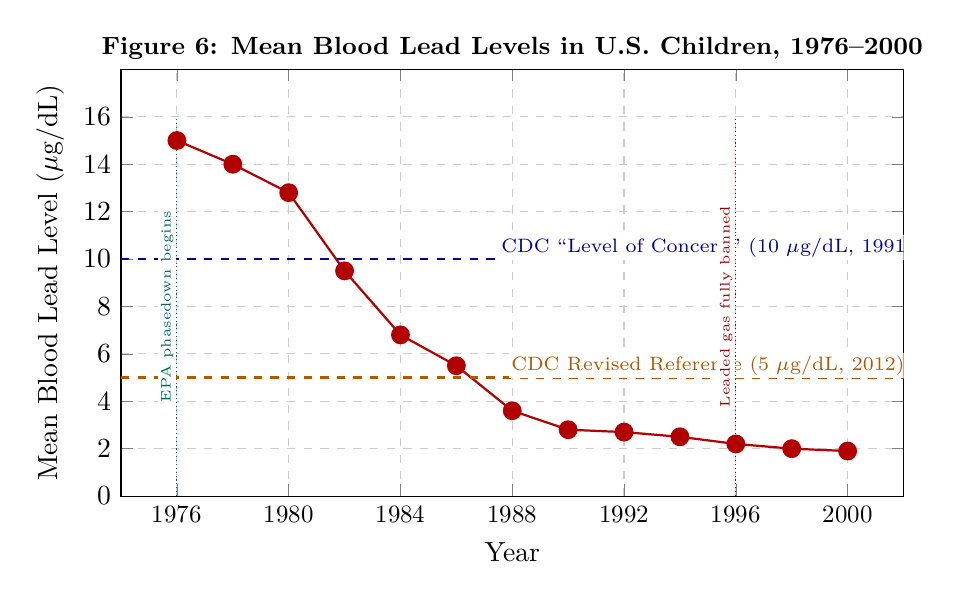
\begin{tikzpicture}
\begin{axis}[
    width=0.95\textwidth,
    height=7cm,
    title={\textbf{Figure 6: Mean Blood Lead Levels in U.S.\ Children, 1976--2000}},
    xlabel={Year},
    ylabel={Mean Blood Lead Level ($\mu$g/dL)},
    xmin=1974, xmax=2002,
    ymin=0, ymax=18,
    xtick={1976,1980,1984,1988,1992,1996,2000},
    xticklabel style={font=\small, /pgf/number format/fixed, /pgf/number format/precision=0, /pgf/number format/1000 sep={}},
    ytick={0,2,4,6,8,10,12,14,16},
    grid=major,
    grid style={dashed, gray!40},
    mark size=3pt,
    every axis title/.style={font=\bfseries\small, at={(0.5,1.05)}},
]
\addplot[thick, red!70!black, mark=*] coordinates {
    (1976, 15.0) (1978, 14.0) (1980, 12.8) (1982, 9.5)
    (1984, 6.8) (1986, 5.5) (1988, 3.6) (1990, 2.8)
    (1992, 2.7) (1994, 2.5) (1996, 2.2) (1998, 2.0) (2000, 1.9)
};
% CDC action level
\draw[dashed, blue!60!black, thick] (axis cs:1974,10) -- (axis cs:2002,10);
\node[font=\scriptsize, blue!60!black, fill=white, inner sep=1pt] at (axis cs:1995,10.5) {CDC ``Level of Concern'' (10 $\mu$g/dL, 1991)};
\draw[dashed, orange!70!black, thick] (axis cs:1974,5) -- (axis cs:2002,5);
\node[font=\scriptsize, orange!70!black, fill=white, inner sep=1pt] at (axis cs:1995,5.5) {CDC Revised Reference (5 $\mu$g/dL, 2012)};
% Policy annotations
\draw[densely dotted, teal!80!black] (axis cs:1976,0) -- (axis cs:1976,16);
\node[rotate=90, anchor=south, font=\tiny, teal!80!black, fill=white, inner sep=1pt] at (axis cs:1976,8) {EPA phasedown begins};
\draw[densely dotted, red!60!black] (axis cs:1996,0) -- (axis cs:1996,16);
\node[rotate=90, anchor=south, font=\tiny, red!60!black, fill=white, inner sep=1pt] at (axis cs:1996,8) {Leaded gas fully banned};
\end{axis}
\end{tikzpicture}\\[0.4em]
% Plain \parbox (not \caption*): avoids wrong automatic ``Figure~\thefigure'' from the float counter
\parbox{\linewidth}{\raggedright\small\emph{Sources: CDC NHANES II (1976--1980), NHANES III (1988--1994), and subsequent survey cycles. Mean blood lead levels in children aged 1--5 dropped from $\sim$15 $\mu$g/dL in 1976 to $\sim$1.9 $\mu$g/dL by 2000---an 87\% decline directly correlated with the EPA-mandated phaseout of leaded gasoline. The generation exposed to $>$10 $\mu$g/dL in the 1960s--1970s reached peak offending age in the late 1980s--early 1990s; the detoxified generation that followed drove the Great Crime Decline.}}
\end{figure}
\FloatBarrier

The national average conceals the racial disparity that is the analytical core of the lead-crime-race nexus. NHANES data disaggregated by race reveals the spatial targeting with devastating clarity.

\begin{figure}[ht]
\centering
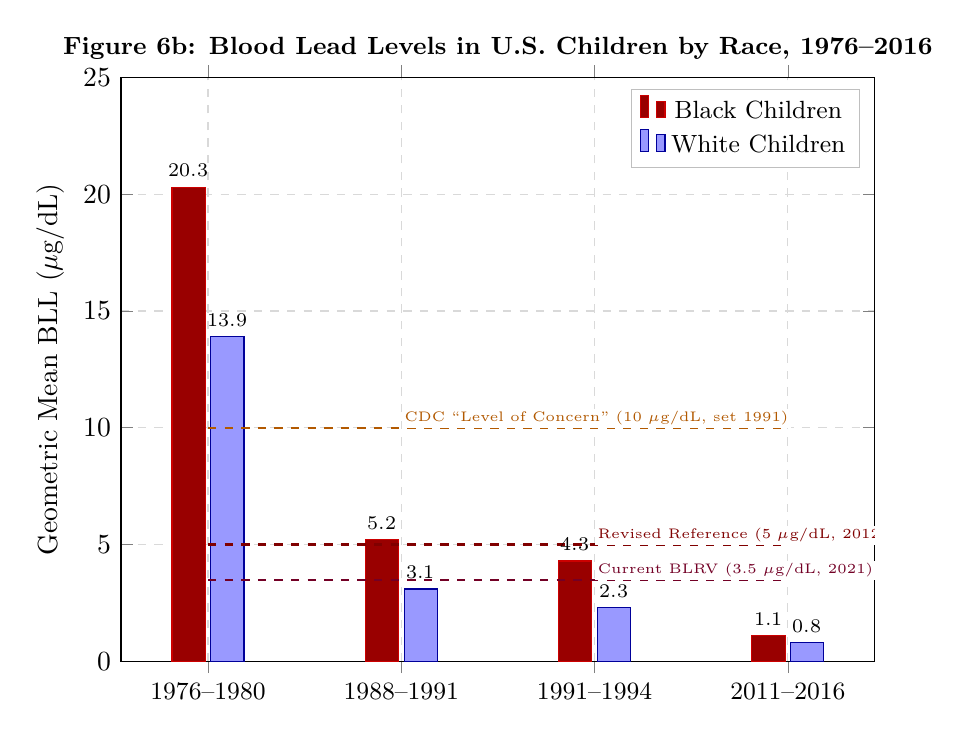
\begin{tikzpicture}
\begin{axis}[
    width=0.92\textwidth,
    height=9cm,
    title={\textbf{Figure 6b: Blood Lead Levels in U.S.\ Children by Race, 1976--2016}},
    ybar,
    bar width=12pt,
    enlarge x limits=0.15,
    ylabel={Geometric Mean BLL ($\mu$g/dL)},
    symbolic x coords={1976--1980,1988--1991,1991--1994,2011--2016},
    xtick=data,
    xticklabel style={font=\small},
    ymin=0, ymax=25,
    grid=major,
    grid style={dashed, gray!30},
    every axis title/.style={font=\bfseries\small, at={(0.5,1.05)}},
    legend style={at={(0.98,0.98)}, anchor=north east, font=\small, draw=gray!50},
    nodes near coords,
    nodes near coords style={font=\scriptsize\bfseries, anchor=south},
]
\addplot[fill=red!60!black, draw=red!80!black] coordinates {
    (1976--1980, 20.3) (1988--1991, 5.2) (1991--1994, 4.3) (2011--2016, 1.1)
};
\addlegendentry{Black Children}

\addplot[fill=blue!40!white, draw=blue!60!black] coordinates {
    (1976--1980, 13.9) (1988--1991, 3.1) (1991--1994, 2.3) (2011--2016, 0.8)
};
\addlegendentry{White Children}

\draw[dashed, orange!70!black, thick] (axis cs:1976--1980,10) -- (axis cs:2011--2016,10);
\node[font=\tiny, orange!70!black, fill=white, inner sep=1pt, anchor=west] at (axis cs:1988--1991,10.4) {CDC ``Level of Concern'' (10 $\mu$g/dL, set 1991)};

\draw[dashed, red!50!black, thick] (axis cs:1976--1980,5) -- (axis cs:2011--2016,5);
\node[font=\tiny, red!50!black, fill=white, inner sep=1pt, anchor=west] at (axis cs:1991--1994,5.4) {Revised Reference (5 $\mu$g/dL, 2012)};

\draw[dashed, purple!60!black, thick] (axis cs:1976--1980,3.5) -- (axis cs:2011--2016,3.5);
\node[font=\tiny, purple!60!black, fill=white, inner sep=1pt, anchor=west] at (axis cs:1991--1994,3.9) {Current BLRV (3.5 $\mu$g/dL, 2021)};

\end{axis}
\end{tikzpicture}\\[0.4em]
\parbox{\linewidth}{\raggedright\small\emph{Sources: CDC NHANES II (1976--1980), NHANES III (1988--1994), and subsequent survey cycles. During peak exposure (1976--1980), Black children carried a geometric mean BLL of 20.3 $\mu$g/dL---46\% higher than White children (13.9) and more than double the CDC's subsequent ``level of concern.'' Both groups far exceeded every safety threshold later established. The disparity narrowed but persisted through 2016 (1.1 vs.\ 0.8). The cohort of Black children measured at 20.3 $\mu$g/dL in the late 1970s is the same population that, 15--20 years later, drove the violent crime surge and the intimate partner homicide plateau documented in the companion analysis. The national average conceals this disparity; the racial disaggregation reveals lead operating as a racially targeted variable.}}
\end{figure}
\FloatBarrier

\begin{figure}[ht]
\centering
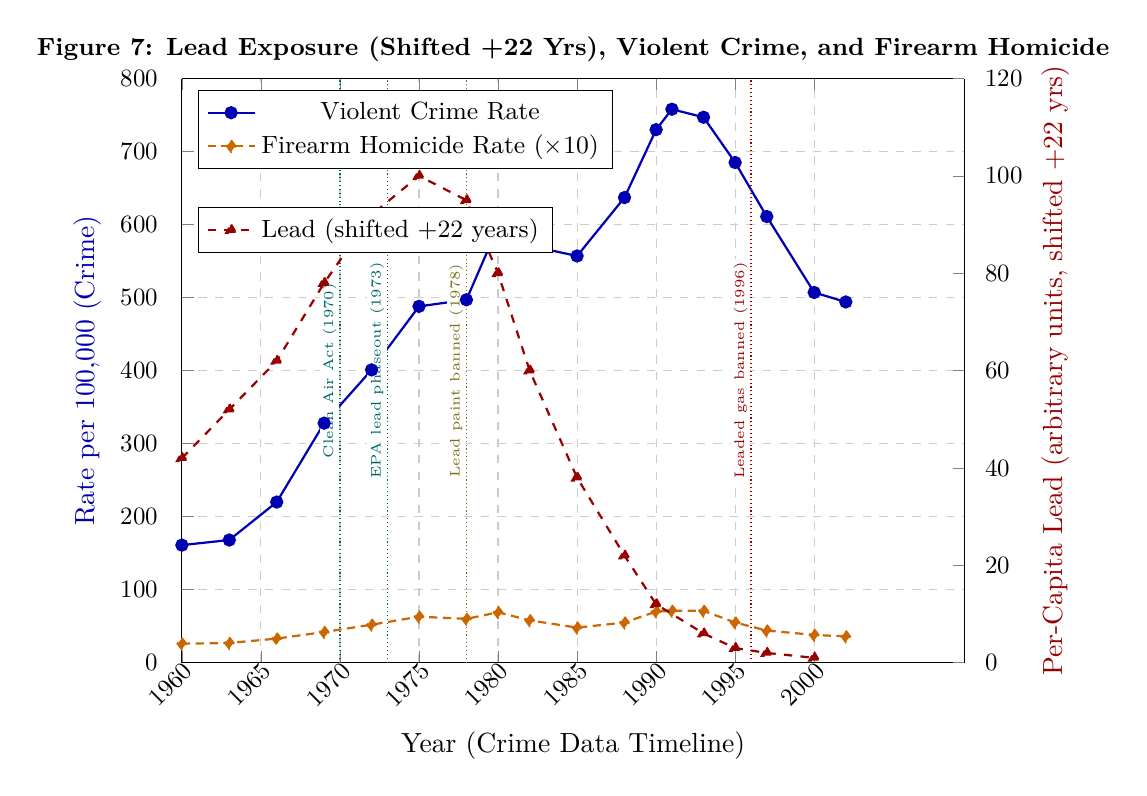
\begin{tikzpicture}
\begin{axis}[
    width=0.95\textwidth,
    height=9cm,
    title={\textbf{Figure 7: Lead Exposure (Shifted +22 Yrs), Violent Crime, and Firearm Homicide}},
    xlabel={Year (Crime Data Timeline)},
    ylabel={Rate per 100{,}000 (Crime)},
    axis y line*=left,
    xmin=1960, xmax=2005,
    enlarge x limits={lower=0.11, upper=0.015},
    ymin=0, ymax=800,
    xtick={1960,1965,1970,1975,1980,1985,1990,1995,2000},
    xticklabel style={rotate=45, anchor=north east, font=\small, yshift=4pt, xshift=4pt, /pgf/number format/fixed, /pgf/number format/precision=0, /pgf/number format/1000 sep={}},
    yticklabel style={font=\small, xshift=-5pt},
    grid=major,
    grid style={dashed, gray!40},
    ylabel style={blue!70!black},
    mark size=2pt,
    every axis title/.style={font=\bfseries\small, at={(0.5,1.05)}},
    legend style={at={(0.02,0.98)}, anchor=north west, font=\small},
]
\addplot[thick, blue!70!black, mark=*] coordinates {
    (1960, 161) (1963, 168) (1966, 220) (1969, 328)
    (1972, 401) (1975, 488) (1978, 497) (1980, 597)
    (1982, 571) (1985, 557) (1988, 637) (1990, 730)
    (1991, 758) (1993, 747) (1995, 685) (1997, 611)
    (2000, 507) (2002, 494)
};
\addlegendentry{Violent Crime Rate}
\addplot[thick, orange!80!black, mark=diamond*, densely dashed] coordinates {
    (1960, 26) (1963, 27) (1966, 33) (1969, 42)
    (1972, 52) (1975, 63) (1978, 60) (1980, 69)
    (1982, 58) (1985, 48) (1988, 55) (1990, 70)
    (1991, 71) (1993, 71) (1995, 55) (1997, 44)
    (2000, 38) (2002, 36)
};
\addlegendentry{Firearm Homicide Rate ($\times$10)}
% Lead policy annotations at mid-graph
\draw[densely dotted, teal!80!black] (axis cs:1970,0) -- (axis cs:1970,800);
\node[rotate=90, anchor=south, font=\tiny, teal!80!black, fill=white, inner sep=1pt] at (axis cs:1970,400) {Clean Air Act (1970)};
\draw[densely dotted, teal!80!black] (axis cs:1973,0) -- (axis cs:1973,800);
\node[rotate=90, anchor=south, font=\tiny, teal!80!black, fill=white, inner sep=1pt] at (axis cs:1973,400) {EPA lead phaseout (1973)};
\draw[densely dotted, olive!80!black] (axis cs:1978,0) -- (axis cs:1978,800);
\node[rotate=90, anchor=south, font=\tiny, olive!80!black, fill=white, inner sep=1pt] at (axis cs:1978,400) {Lead paint banned (1978)};
\draw[densely dotted, red!60!black] (axis cs:1996,0) -- (axis cs:1996,800);
\node[rotate=90, anchor=south, font=\tiny, red!60!black, fill=white, inner sep=1pt] at (axis cs:1996,400) {Leaded gas banned (1996)};
\end{axis}
\begin{axis}[
    width=0.95\textwidth,
    height=9cm,
    axis y line*=right,
    axis x line=none,
    ylabel={Per-Capita Lead (arbitrary units, shifted +22 yrs)},
    xmin=1960, xmax=2005,
    enlarge x limits={lower=0.11, upper=0.015},
    ymin=0, ymax=120,
    ylabel style={red!60!black},
    yticklabel style={font=\small, xshift=4pt},
    mark size=2pt,
    legend style={at={(0.02,0.78)}, anchor=north west, font=\small},
]
\addplot[thick, red!60!black, mark=triangle*, dashed] coordinates {
    (1960, 42) (1963, 52) (1966, 62) (1969, 78)
    (1972, 92) (1975, 100) (1978, 95) (1980, 80)
    (1982, 60) (1985, 38) (1988, 22) (1990, 12)
    (1993, 6) (1995, 3) (1997, 2) (2000, 1)
};
\addlegendentry{Lead (shifted +22 years)}
\end{axis}
\end{tikzpicture}\\[0.4em]
% Plain \parbox (not \caption*): avoids wrong ``Figure~\thefigure'' under the plot; number stays in axis title only
\parbox{\linewidth}{\raggedright\small\emph{Sources: Nevin, Environmental Research 104 (2007); Reyes, NBER Working Paper 13097 (2007); EPA; FBI UCR; CDC WONDER. Lead data shifted +22 years; firearm homicide scaled $\times$10. Both crime curves track the lagged lead-exposure curve with striking fidelity, declining as the detoxified generation ages into adulthood.}}
\end{figure}

\subsection{\texorpdfstring{\textbf{The Multi-Vector Containment: Lead
in Water, Schools, and the Property-Tax
Trap}}{The Multi-Vector Containment: Lead in Water, Schools, and the Property-Tax Trap}}\label{the-multi-vector-containment-lead-in-water-schools-and-the-property-tax-trap}

The preceding analysis establishes the catastrophic scale of aerosolized
lead from automotive fuel. However, the atmosphere was not the only
delivery mechanism. A comprehensive accounting reveals that lead
exposure operated through at least three simultaneous vectors---air,
residential water, and institutional plumbing---all concentrated by the
same property-tax funding architecture that sorts infrastructure quality
by race and wealth. The highway was one barrel of a multi-barreled
weapon.

\subsubsection{\texorpdfstring{\textbf{Lead Service Lines: The Pipe in
the Wall}}{Lead Service Lines: The Pipe in the Wall}}\label{lead-service-lines-the-pipe-in-the-wall}

Lead pipes were the standard material for residential water service
lines from the 1880s through the mid-twentieth century. Many
municipalities continued installing them well into the 1980s; Chicago,
notably, \emph{required} lead service lines by municipal plumbing code
until federal legislation intervened. The 1986 amendments to the Safe
Drinking Water Act (SDWA) banned the use of lead pipes and lead solder
in public water systems, though the statutory definition of
``lead-free'' was not tightened from 8 percent to 0.25 percent lead
content until the Reduction of Lead in Drinking Water Act of 2011,
effective 2014.\\
The legacy infrastructure remains staggering. As of the early 2020s, the
EPA and the Natural Resources Defense Council estimated that between
\textbf{9.2 and 12.8 million lead service lines} remain in active use
across the United States. The EPA's revised Lead and Copper Rule (LCRR),
finalized in October 2024, requires utilities to inventory and begin
replacing these lines within a ten-year compliance window, though
funding remains bitterly contested.\\
The racial geography of this infrastructure is not accidental. A 2022
study by Switzer and Teodoro, published in the \emph{Proceedings of the
National Academy of Sciences}, demonstrated that communities with higher
proportions of Black and Latino residents were significantly more likely
to retain lead service lines and significantly less likely to have
initiated replacement programs. This finding aligns with decades of EPA
environmental justice data showing that nonwhite and low-income
communities bear disproportionate burdens of infrastructure neglect
across every measurable dimension.\\
The catastrophe in Flint, Michigan, crystallized this dynamic into a
national scandal. In April 2014, when the city switched its water source
to the Flint River without implementing corrosion control treatment, lead
leached from the city's aging service lines into the drinking water
supply. A landmark study by Hanna-Attisha and colleagues, published in
the \emph{American Journal of Public Health} (2016), demonstrated that
blood lead levels in children under five nearly doubled in
high-exposure zip codes following the switch. Twelve residents died from
Legionnaires' disease linked to the same contaminated water system.
Flint's population was approximately 57 percent Black, with a poverty
rate exceeding 40 percent---a textbook convergence of racial segregation,
fiscal austerity, and environmental poisoning.\\
The critical insight is that Flint was not an aberration; it was a
\emph{visible} instance of a condition that persists invisibly in
thousands of municipalities. The same children who breathed aerosolized
lead from highway traffic drank lead-contaminated water from the pipes
in their homes.

\subsubsection{\texorpdfstring{\textbf{Lead in Schools: The Unregulated
Vector}}{Lead in Schools: The Unregulated Vector}}\label{lead-in-schools-the-unregulated-vector}

If lead in residential water constitutes neglect, lead in school water
constitutes institutional poisoning of children in state custody.
Remarkably, the EPA \textbf{does not regulate lead in school drinking
water} under the Safe Drinking Water Act, because most schools are not
classified as public water systems. Testing is voluntary in the majority
of states, and remediation is unfunded.\\
A 2018 report by the U.S. Government Accountability Office
(GAO-18-382) revealed the scale of this regulatory void: of the school
districts surveyed, only \textbf{43 percent had tested for lead in
their drinking water at all}. Of those that did test, \textbf{37
percent found elevated lead levels} in at least some fixtures---drinking
fountains, kitchen faucets, bathroom sinks. The GAO estimated that
millions of American children attend schools where lead testing has
never been conducted.\\
The critical variable is building age. Schools constructed before 1986
are far more likely to contain lead solder in their plumbing joints,
brass fixtures with high lead content, and in some cases lead service
lines connecting them to the municipal supply. A 2019 study by Dor\'{e}
and colleagues at the Harvard T.H. Chan School of Public Health,
published in \emph{Environmental Science \& Technology}, documented that
older plumbing fixtures in schools contributed significantly to
first-draw lead concentrations, particularly after weekends and vacation
periods when water sits stagnant in the pipes, maximizing leaching
time.\\
This is where the property-tax architecture becomes lethal.

\subsubsection{\texorpdfstring{\textbf{The Property-Tax Feedback Loop:
Funding Segregation Through
Infrastructure}}{The Property-Tax Feedback Loop: Funding Segregation Through Infrastructure}}\label{the-property-tax-feedback-loop}

The United States funds approximately 45 percent of K--12 education
through local revenue sources, predominantly property taxes (National
Center for Education Statistics). This funding architecture, upheld by
the Supreme Court in \emph{San Antonio Independent School District v.
Rodriguez} (1973), ensures that per-pupil spending is a direct function
of neighborhood property values. The resulting disparities are not
marginal: per-pupil spending gaps between wealthy and poor districts
within the same state can exceed ratios of 3:1 (Baker,
\emph{Educational Inequality and School Finance}, 2018).\\
Capital expenditures---building maintenance, plumbing remediation, HVAC
replacement---are among the first casualties of chronic underfunding.
The American Society of Civil Engineers' 2021 Infrastructure Report Card
assigned U.S.\ school infrastructure a grade of \textbf{D+}, estimating
an \textbf{\$85 billion national funding gap} concentrated
overwhelmingly in high-poverty districts. A 2020 report by the 21st
Century School Fund and the National Council on School Facilities
confirmed that predominantly nonwhite districts received significantly
less capital investment per student than their white counterparts.\\
The result is a self-reinforcing feedback loop of extraordinary
cruelty. The same neighborhoods that were redlined in the 1930s---locked
into artificially depressed property values by state-mandated
disinvestment---generate the lowest property-tax revenues. Those
revenues fund the most decrepit school buildings. Those buildings contain
the oldest plumbing. That plumbing leaches lead into the drinking water
of children who are already breathing aerosolized lead from the highways
routed through their neighborhoods and drinking lead-contaminated water
from the pipes in their homes. When those schools visibly deteriorate,
neighborhood property values decline further (Cellini, Ferreira, \&
Rothstein, \emph{Journal of Public Economics}, 2010), shrinking the tax
base, further starving capital budgets, and ensuring that the lead pipes
will never be replaced.\\
The districts too poor to replace aging plumbing are too poor to test
for contamination, and too poor to remediate when contamination is
found. The children poisoned in these schools are the same children
poisoned in their homes and on their streets. Three vectors, one target
population, one funding mechanism ensuring that the harm is
simultaneously inflicted and perpetuated.

\FloatBarrier

\begin{figure}[ht]
\centering
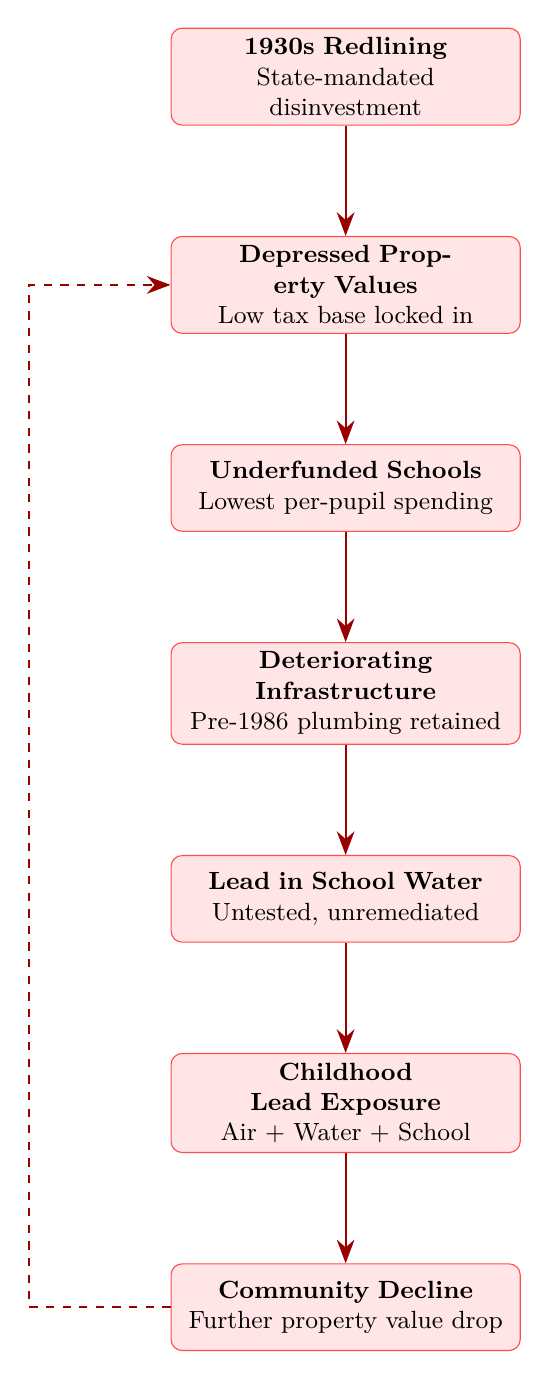
\begin{tikzpicture}[
    node distance=1.4cm,
    every node/.style={font=\small},
    block/.style={rectangle, draw=red!70, fill=red!10, text width=4.2cm,
                  align=center, rounded corners, minimum height=1.1cm},
    arrow/.style={-{Stealth[length=3mm]}, thick, red!60!black},
]
\node[block] (redline) {\textbf{1930s Redlining}\\State-mandated\\disinvestment};
\node[block, below=of redline] (propval) {\textbf{Depressed Property Values}\\Low tax base locked in};
\node[block, below=of propval] (funding) {\textbf{Underfunded Schools}\\Lowest per-pupil spending};
\node[block, below=of funding] (infra) {\textbf{Deteriorating Infrastructure}\\Pre-1986 plumbing retained};
\node[block, below=of infra] (lead) {\textbf{Lead in School Water}\\Untested, unremediated};
\node[block, below=of lead] (children) {\textbf{Childhood Lead Exposure}\\Air + Water + School};
\node[block, below=of children] (decline) {\textbf{Community Decline}\\Further property value drop};
\draw[arrow] (redline) -- (propval);
\draw[arrow] (propval) -- (funding);
\draw[arrow] (funding) -- (infra);
\draw[arrow] (infra) -- (lead);
\draw[arrow] (lead) -- (children);
\draw[arrow] (children) -- (decline);
\draw[arrow, dashed] (decline.west) -- +(-1.8,0) |- (propval.west);
\end{tikzpicture}
\caption*{\textbf{Figure 8: The Property-Tax Feedback Loop}\\[0.3cm]
\emph{Redlining depresses property values, which starves school funding, which preserves lead infrastructure, which poisons children, which deepens community decline, which further depresses property values. The dashed arrow represents the recursive, self-reinforcing nature of the cycle. Sources: NCES; ASCE Infrastructure Report Card (2021); GAO-18-382 (2018); Cellini et al., \emph{Journal of Public Economics} (2010).}}
\label{fig:property-tax-feedback}
\end{figure}

\FloatBarrier

\subsection{\texorpdfstring{\textbf{Spatial Weaponry: Intentional
Highway Routing and the Calculus of Systemic
Racism}}{Spatial Weaponry: Intentional Highway Routing and the Calculus of Systemic Racism}}\label{spatial-weaponry-intentional-highway-routing-and-the-calculus-of-systemic-racism}

If the petroleum industry manufactured the neurotoxin, the state
manufactured the distribution network that ensured marginalized
populations absorbed the heaviest biological burden. The violent crime
wave was not uniformly distributed across the United States; it was
hyper-concentrated in inner-city, minority neighborhoods. This localized
intensity was not a cultural anomaly, but the direct, mathematically
predictable output of state-sponsored spatial engineering, primarily
executed through the Federal-Aid Highway Act of 1956.

\subsubsection{\texorpdfstring{\textbf{The Architecture of
Vulnerability:
Redlining}}{The Architecture of Vulnerability: Redlining}}\label{the-architecture-of-vulnerability-redlining}

The targeted vulnerability of these communities began in the 1930s with
the Home Owners' Loan Corporation (HOLC), which created residential
security maps that systematically ``redlined'' neighborhoods based
almost entirely on their racial and ethnic composition. Neighborhoods
containing Black or immigrant populations were graded as ``hazardous''
and deliberately cut off from federal mortgage backing, private capital,
and the primary mechanism of American wealth generation: homeownership.
Over the subsequent decades, this state-mandated disinvestment locked
these communities into isolated zones of concentrated poverty,
deteriorating housing, and failing infrastructure, entirely stripping
them of the economic and political capital necessary to defend
themselves against future incursions.

\subsubsection{\texorpdfstring{\textbf{The Federal-Aid Highway Act of
1956 and ``Slum
Clearance''}}{The Federal-Aid Highway Act of 1956 and ``Slum Clearance''}}\label{the-federal-aid-highway-act-of-1956-and-slum-clearance}

When the Federal-Aid Highway Act of 1956 was signed by President Dwight
D. Eisenhower, authorizing the construction of a 41,000-mile interstate
network, it was aggressively weaponized by urban planners as a tool for
racial segregation and targeted ``slum clearance''. Government officials
and planners---most notoriously Robert Moses in New York
City---deliberately routed massive, federally funded expressways
directly through the heart of thriving Black and brown communities.\\
The physical and social devastation was absolute. The routing of these
massive concrete arteries destroyed homes, dismantled social cohesion,
eradicated local businesses, and erected physical barriers that
permanently separated minority populations from transit, healthcare, and
economic mobility. Examples of this intentional destruction span the nation:

\begin{itemize}
\tightlist
\item
  \textbf{New York City (Cross-Bronx Expressway):} Robert Moses'
  Cross-Bronx Expressway severed the Bronx, displacing thousands of
  families and leaving a permanent legacy of respiratory disease and
  economic devastation. Moses notoriously stated that ``our categorical
  imperative is action to clear the slums'' and that minorities could
  not be allowed to dictate or hinder this progress.\\
\item
  \textbf{Syracuse, New York (15th Ward):} The 15th Ward served as a
  historic refuge for Black Southerners migrating north. Following years
  of federally mandated redlining that deterred private investment, the
  city declared the neighborhood ``blighted''. City officials chose to
  route the elevated I-81 viaduct directly through the ward, displacing
  over 1,300 families and physically cementing the separation between
  impoverished Black urban residents and affluent white suburbanites.
  The neighborhood housed 90\% of the city's Black population.\\
\item
  \textbf{New Orleans (Claiborne Expressway):} The Claiborne
  Expressway, dubbed ``The Monster,'' decimated the historic Tremé
  neighborhood, one of the oldest free Black communities in the United
  States.\\
\item
  \textbf{Miami, Florida (Overtown):} In the 1950s, the Overtown
  neighborhood was the thriving cultural and economic center of Black
  Miami, often referred to as the ``Harlem of the South.'' Early
  engineering proposals for Interstate 95 suggested routing the highway
  along an abandoned railway line, a trajectory that would have left
  Overtown entirely untouched. However, planners summarily rescinded
  this proposal without holding a single public hearing in the affected
  community. Driven by explicit, documented desires to ``reclaim
  Overtown's land for development'' and ensure the ``continued whiteness
  of central Miami,'' officials routed the massive I-95/I-395
  interchange directly through the center of the neighborhood. The
  construction obliterated 40 square blocks, displaced over 10,000
  people, and decimated the community's economic independence.\\
\item
  \textbf{Nashville, Tennessee (I-40):} Early highway plans considered
  routes that would have encroached upon the exclusive, affluent white
  enclave of Belle Meade and the Vanderbilt University area. State
  planners quickly abandoned these proposals, recognizing that
  condemning land from prominent white citizens would be both
  exorbitantly expensive and ``political suicide.'' Instead, Nashville
  planners deliberately altered the trajectory of Interstate 40 to
  bisect the city's main Black business district, permanently walling
  off historically Black institutions---such as Fisk University and
  Meharry Medical College---from the communities they had served for
  generations.\\
\item
  \textbf{Baltimore, Maryland (The Highway to Nowhere):} The Franklin
  and Mulberry streets corridor was identified in 1944 by notorious
  highway builder Robert Moses specifically because it was the ``path
  of least resistance''---meaning it was low-income and predominantly
  Black. The resulting expressway demolished vibrant Black neighborhoods
  while serving primarily white suburban automobile commuters.
\end{itemize}

The 1944 ``Interregional Highways'' report, which laid the groundwork
for the 1956 Act, explicitly called for freeways to cut through the
center of major cities to eradicate ``blighted areas'' and
``slums''---terms that were universally understood as coded proxies for
Black neighborhoods. Similarly, the Underwriting Manual of the Federal
Housing Administration openly advocated for using highways to physically
separate African-American neighborhoods from White neighborhoods.
Nationally, this state-sponsored infrastructure project resulted in the
displacement of over one million people, predominantly minorities, while
simultaneously subsidizing ``white flight'' to the suburbs.

\begin{figure}[ht]
\centering
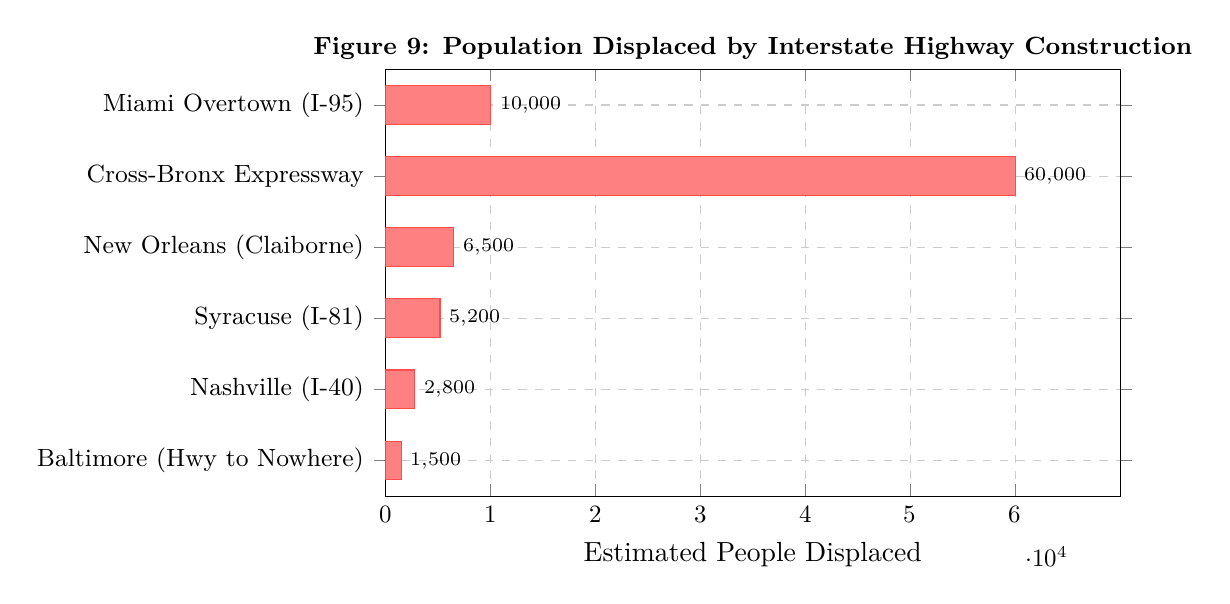
\begin{tikzpicture}
\begin{axis}[
    width=0.9\textwidth,
    height=7cm,
    title={\textbf{Figure 9: Population Displaced by Interstate Highway Construction}},
    xbar,
    bar width=14pt,
    xlabel={Estimated People Displaced},
    symbolic y coords={{Baltimore (Hwy to Nowhere)},{Nashville (I-40)},{Syracuse (I-81)},{New Orleans (Claiborne)},{Cross-Bronx Expressway},{Miami Overtown (I-95)}},
    ytick=data,
    yticklabel style={font=\small},
    xmin=0, xmax=70000,
    xtick={0,10000,20000,30000,40000,50000,60000},
    xticklabel style={font=\small},
    grid=major,
    grid style={dashed, gray!40},
    every axis title/.style={font=\bfseries\small, at={(0.5,1.05)}},
    nodes near coords,
    nodes near coords style={font=\scriptsize\bfseries, anchor=west},
]
\addplot[fill=red!50, draw=red!70] coordinates {
(1500,{Baltimore (Hwy to Nowhere)})
(2800,{Nashville (I-40)})
(5200,{Syracuse (I-81)})
(6500,{New Orleans (Claiborne)})
(60000,{Cross-Bronx Expressway})
(10000,{Miami Overtown (I-95)})
};
\end{axis}
\end{tikzpicture}
\caption*{\emph{Sources: AARP, ``Decades of Highway Construction and Community Destruction'' (2023); Vanderbilt University, ``White Men's Roads Through Black Men's Homes'' (2020); ACLU; Baltimore Magazine; city-level historical records. Nationally, over one million people---predominantly Black and minority residents---were displaced by interstate highway construction. These figures represent direct residential displacement only and do not capture the broader economic destruction, loss of social networks, or generational wealth erasure.}}
\end{figure}

\begin{figure}[ht]
\centering
\includegraphics[width=0.95\textwidth]{Philadelphia_gun_red.jpeg}
\caption*{\textbf{Figure 10: HOLC Redlining Grades (1930s) Overlaid with Firearm Homicide Density --- Philadelphia, PA}\\[0.3cm]
\emph{HOLC residential security grades: Grade A (green/``Best''), Grade B (blue/``Still Desirable''), Grade C (yellow/``Definitely Declining''), Grade D (red/``Hazardous''). Firearm homicide incidents overlaid as purple/orange density clusters. The spatial coincidence between Grade D zones and the highest-density homicide clusters demonstrates the multi-decade pipeline from state-mandated disinvestment to concentrated lethal violence. Interstate highways (I-76, I-95, I-676) were subsequently routed through these same redlined corridors, concentrating neurotoxic lead exhaust onto populations already trapped by capital starvation. Sources: University of Richmond, Mapping Inequality; OpenDataPhilly.}}
\end{figure}

\subsubsection{\texorpdfstring{\textbf{Addressing the ``Smoking Gun'':
The Intentionality of Toxic
Exposure}}{Addressing the ``Smoking Gun'': The Intentionality of Toxic Exposure}}\label{addressing-the-smoking-gun-the-intentionality-of-toxic-exposure}

The routing of these highways had a profound, insidious secondary
effect: it transformed these redlined neighborhoods into concentrated
sacrifice zones of toxic exposure. Because these highways carried
hundreds of thousands of vehicles burning TEL-infused fuel daily, the
surrounding marginalized communities were subjected to a relentless
bombardment of aerosolized lead exhaust, fine particulate matter
(PM2.5), and diesel emissions.\\
When analyzing the historical intentionality of this poisoning, a
critical distinction must be made between the intent to segregate and
the explicit intent to poison. Research indicates there is no single
``smoking gun'' memo wherein government officials explicitly stated an
intention to \emph{poison} Black communities specifically with lead
exhaust. The absence of such a document in the historical
record---unlike the highly explicit internal corporate documents
regarding the dangers of lead paint or the ``loony gas''
disasters---often frustrates legal attempts to prove intentional
discrimination under the Fourteenth Amendment's Equal Protection Clause,
which requires an exceptionally high burden of discriminatory intent.\\
However, the lack of a ``poisoning memo'' does not absolve the state of
intentional, systematic harm. The intent to racially segregate,
displace, and economically destroy these communities was explicit,
undeniable, and highly documented in the urban planning doctrines of the
era. The 1944 ``Interregional Highways'' report, which laid the
groundwork for the 1956 Act, explicitly called for freeways to cut
through the center of major cities to eradicate ``blighted areas'' and
``slums''---terms that were universally understood as coded proxies for
Black neighborhoods. Similarly, the Underwriting Manual of the Federal
Housing Administration openly advocated for using highways to physically
separate African-American neighborhoods from White neighborhoods.
Planners like Robert Moses were well aware that they were introducing
massive, highly polluting industrial thoroughfares into dense
residential areas; Moses notoriously stated that ``our categorical
imperative is action to clear the slums'' and that minorities could not
be allowed to dictate or hinder this progress.\\
The government and the planners knew, via the 1925 Surgeon General's
conference and ongoing public health debates, that automotive exhaust
contained toxic lead. Simultaneously, they explicitly and intentionally
routed the highest concentrations of that exhaust directly through Black
communities. The resulting environmental pollution, toxic waste
distribution, and horrific public health outcomes---including severe
asthma, cardiovascular disease, and chronic lead poisoning---were
accepted as collateral damage inflicted upon populations deemed
politically expendable.\\
Today, modern geospatial analysis and soil sampling confirm the
devastating legacy of this spatial weaponry. Historically redlined
neighborhoods possess reservoirs of toxic lead dust in their soils that
are vastly higher than in non-redlined areas, exposing residents to
rates of air pollution and lead contamination that are up to five times
higher than in integrated communities. Because children in these
specific neighborhoods absorbed vastly disproportionate amounts of
environmental lead from the highways intentionally placed beside their
homes, they were biologically handicapped before they even reached
adolescence. They suffered from the exact neurological deficits and
prefrontal cortex damage that precipitate aggression and violence.
Therefore, the state's intentional spatial engineering directly
guaranteed that minority communities would suffer the most severe
biological consequences of the petroleum industry's neurotoxin.

\subsection{\texorpdfstring{\textbf{The Fourteenth Amendment and the
Jurisprudence of
Intent}}{The Fourteenth Amendment and the Jurisprudence of Intent}}\label{the-fourteenth-amendment-and-the-jurisprudence-of-intent}

Despite the overwhelming historical evidence that infrastructure
projects were utilized to intentionally segregate, poison, and dismantle
Black communities, the American judicial system has largely shielded
these state actions from constitutional accountability. For racial
justice advocates seeking to prove that highway routing constitutes
\emph{de jure} segregation or actionable environmental racism, the legal
architecture of the Fourteenth Amendment presents a nearly
insurmountable jurisprudential barrier.

\subsubsection{\texorpdfstring{\textbf{The Insurmountable Burden of
``Discriminatory
Intent''}}{The Insurmountable Burden of ``Discriminatory Intent''}}\label{the-insurmountable-burden-of-discriminatory-intent}

The analytical gap between historical reality and constitutional law
hinges entirely on how the federal judiciary defines discrimination.
Under the Equal Protection Clause of the Fourteenth Amendment, a
government action is not unconstitutional simply because it produces a
severe, racially disproportionate impact. Following the Supreme Court's
landmark decisions in \emph{Washington v. Davis} (1976) and
\emph{Village of Arlington Heights v. Metropolitan Housing Development
Corp.} (1977), plaintiffs must prove that the state action was
explicitly motivated by ``discriminatory intent'' or racial animus.\\
To establish this intent, the Court in \emph{Arlington Heights} outlined
a framework of circumstantial evidentiary factors, including the
historical background of the decision, significant departures from
normal administrative procedures, and the legislative history. In
theory, this allows plaintiffs to build a circumstantial case. In
practice, however, the federal courts have applied this standard so
rigidly that it effectively requires a ``smoking gun''---a memo, a
recorded statement, or an overt admission by a government official that
a highway was routed through a Black community specifically
\emph{because} of racial hatred.\\
Because mid-century urban planners, highway engineers, and politicians
were highly adept at laundering their racial motivations through the
sanitized, race-neutral language of ``traffic efficiency,'' ``urban
renewal,'' and ``blight removal,'' such smoking guns rarely exist. The
intent standard effectively limits the Fourteenth Amendment to policing
overt, individual acts of malice, rendering the Constitution entirely
blind to the structural, systemic racism that engineered the interstate
highway system and forced toxic pollution onto marginalized groups.

{\def\LTcaptype{none} % do not increment counter
\begin{longtable}[]{@{}
  >{\raggedright\arraybackslash}p{(\linewidth - 2\tabcolsep) * \real{0.5000}}
  >{\raggedright\arraybackslash}p{(\linewidth - 2\tabcolsep) * \real{0.5000}}@{}}
\toprule\noalign{}
\begin{minipage}[b]{\linewidth}\raggedright
The \emph{Arlington Heights} Factors for Proving Discriminatory Intent
\end{minipage} & \begin{minipage}[b]{\linewidth}\raggedright
Application to Mid-Century Interstate Highway Routing
\end{minipage} \\
\midrule\noalign{}
\endhead
\bottomrule\noalign{}
\endlastfoot
\textbf{Disproportionate Impact} & Clear and undeniable. Highways
disproportionately displaced Black residents and hyper-concentrated
vehicular pollution. (Legally insufficient alone to prove an Equal
Protection violation). \\
\textbf{Historical Background} & A deep legacy of state-sponsored
redlining (HOLC maps) preceded highway placement, artificially
depressing land values to justify ``slum clearance.'' \\
\textbf{Departures from Normal Procedures} & Highly prevalent. Planners
routinely canceled public hearings in Black neighborhoods (e.g.,
Overtown, Miami) or ignored established routing criteria that favored
preserving intact neighborhoods. \\
\textbf{Contemporary Statements} & Extremely rare, making the ``smoking
gun'' burden nearly impossible. When they do exist (e.g., Miami planners
explicitly citing the goal of maintaining the ``whiteness of central
Miami''), courts still struggle to apply broad structural remedies. \\
\end{longtable}
}

\begin{figure}[htbp]
\centering
% \makebox centers the tight TikZ bbox in \linewidth (avoids a visually left-heavy diagram)
\makebox[\linewidth][c]{%
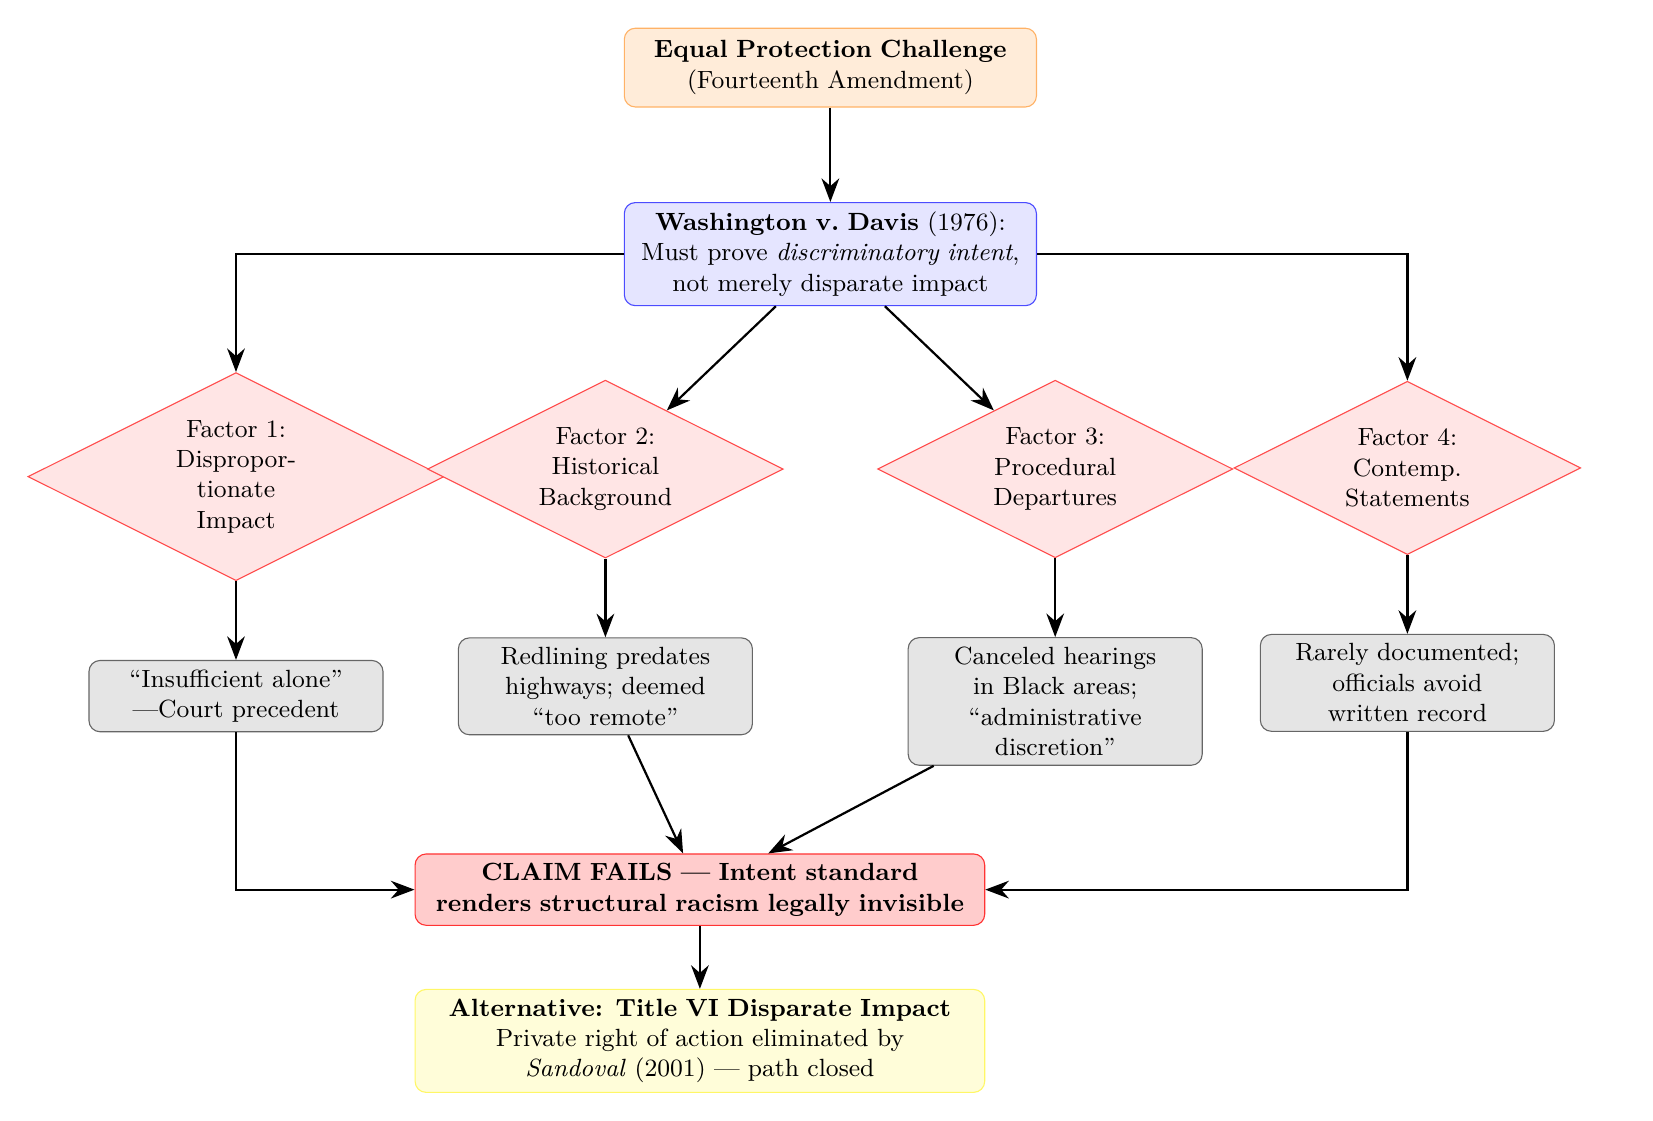
\begin{tikzpicture}[
    node distance=1.2cm and 0.8cm,
    every node/.style={font=\small},
    decision/.style={diamond, draw=red!70, fill=red!10, text width=2.2cm, align=center, inner sep=1pt, aspect=2},
    block/.style={rectangle, draw=blue!70, fill=blue!10, text width=3.8cm, align=center, rounded corners, minimum height=1cm},
    result/.style={rectangle, draw=black!60, fill=gray!20, text width=3.5cm, align=center, rounded corners, minimum height=0.8cm},
    fail/.style={rectangle, draw=red!80, fill=red!20, text width=3.5cm, align=center, rounded corners, minimum height=0.8cm, font=\small\bfseries},
    arrow/.style={-{Stealth[length=3mm]}, thick},
]

% Top node
\node[block, text width=5cm, fill=orange!15, draw=orange!60] (start) {\textbf{Equal Protection Challenge}\\(Fourteenth Amendment)};

% Requirement
\node[block, below=of start, text width=5cm] (req) {\textbf{Washington v.\ Davis} (1976):\\Must prove \emph{discriminatory intent},\\not merely disparate impact};

% Four factors
\node[decision, below left=1.5cm and 3.6cm of req] (f1) {Factor 1:\\Dispropor-\\tionate\\Impact};
% Negative lateral shift pulls Factor 2 right and Factor 3 left so the pair sits tighter
\node[decision, below left=1.5cm and -0.9cm of req] (f2) {Factor 2:\\Historical\\Background};
\node[decision, below right=1.5cm and -0.9cm of req] (f3) {Factor 3:\\Procedural\\Departures};
\node[decision, below right=1.5cm and 3.6cm of req] (f4) {Factor 4:\\Contemp.\\Statements};

% Outcomes for each
\node[result, below=1cm of f1] (r1) {``Insufficient alone''\\---Court precedent};
\node[result, below=1cm of f2] (r2) {Redlining predates\\highways; deemed\\``too remote''};
\node[result, below=1cm of f3] (r3) {Canceled hearings\\in Black areas;\\``administrative\\discretion''};
\node[result, below=1cm of f4] (r4) {Rarely documented;\\officials avoid\\written record};

% Final outcome
\node[fail, below=1.5cm of r2, text width=7cm, xshift=1.2cm] (final) {CLAIM FAILS --- Intent standard\\renders structural racism legally invisible};

% Title VI alternative
\node[block, below=0.8cm of final, text width=7cm, fill=yellow!15, draw=yellow!60] (titlevi) {\textbf{Alternative: Title VI Disparate Impact}\\Private right of action eliminated by\\\emph{Sandoval} (2001) --- path closed};

% Arrows
\draw[arrow] (start) -- (req);
\draw[arrow] (req) -| (f1);
\draw[arrow] (req) -- (f2);
\draw[arrow] (req) -- (f3);
\draw[arrow] (req) -| (f4);
\draw[arrow] (f1) -- (r1);
\draw[arrow] (f2) -- (r2);
\draw[arrow] (f3) -- (r3);
\draw[arrow] (f4) -- (r4);
\draw[arrow] (r1) |- (final);
\draw[arrow] (r2) -- (final);
\draw[arrow] (r3) -- (final);
\draw[arrow] (r4) |- (final);
\draw[arrow] (final) -- (titlevi);
% Outer columns + |- paths extend the bbox further left than right; pad east so the block centers on the page
\path let \p1=(current bounding box.south east), \p2=(current bounding box.north east) in (\x1+16pt,\y1) (\x2+16pt,\y2);

\end{tikzpicture}%
}
\caption*{\textbf{Figure 11: The Impossibility of Proving Discriminatory Intent Under \emph{Arlington Heights}}\\[0.3cm]
\emph{Decision flowchart illustrating the practical impossibility of proving discriminatory intent under the \emph{Arlington Heights} framework as applied to mid-century infrastructure routing. Each of the four evidentiary factors is either legally insufficient standing alone or functionally unobtainable, creating a hermetically sealed legal shield for structurally racist state action. The alternative Title VI disparate impact pathway was foreclosed by \emph{Sandoval} (2001). Sources: \emph{Washington v.\ Davis}, 426 U.S.\ 229 (1976); \emph{Village of Arlington Heights v.\ MHDC}, 429 U.S.\ 252 (1977); \emph{Alexander v.\ Sandoval}, 532 U.S.\ 275 (2001).}}
\label{fig:arlington-heights-flowchart}
\end{figure}

\subsubsection{\texorpdfstring{\textbf{The Atwater Confession and the
Proxy Variable
Problem}}{The Atwater Confession and the Proxy Variable Problem}}\label{the-atwater-confession-and-the-proxy-variable-problem}

The intent standard's fatal deficiency is not merely that it is
difficult to satisfy---it is that it was designed to be satisfied only
by the crude, obsolete forms of racism that the political establishment
had already abandoned. The most devastating proof of this structural
blindness comes not from legal scholarship, but from the architects of
the strategy themselves.\\
On October 26, 1981, Republican political strategist Lee Atwater---then
serving as Deputy Assistant to President Reagan for Political Affairs,
and later campaign manager for George H.W. Bush's 1988 presidential
campaign and chairman of the Republican National Committee---gave an
anonymous interview to political scientist Alexander P. Lamis, who was
conducting research for his book \emph{The Two-Party South} (Oxford
University Press, 1984). Lamis published the quotes anonymously;
Atwater's identity was not confirmed until after his death in 1991, when
Lamis revealed it in the 1999 revised edition of the work. The full
audio was made publicly available in 2012 by James Carter IV, provided
to \emph{The Nation}.\\
Atwater's statement constitutes a frank admission of deliberate variable
substitution in racial politics:

\begin{quote}
You start out in 1954 by saying, ``N----r, n----r, n----r.'' By 1968
you can't say ``n----r''---that hurts you, backfires. So you say stuff
like, uh, forced busing, states' rights, and all that stuff, and you're
getting so abstract. Now, you're talking about cutting taxes, and all
these things you're talking about are totally economic things and a
byproduct of them is, blacks get hurt worse than whites\ldots\ ``We want
to cut this,'' is much more abstract than even the busing thing, uh, and
a hell of a lot more abstract than ``N----r, n----r.''
\end{quote}

\noindent The analytical significance of this passage cannot be
overstated. Atwater is not speculating about political strategy; he is
describing the operational mechanics of a deliberate encoding process.
The explicit racial variable---direct invocation of racial
slurs---became politically costly, so the political apparatus replaced it
with \textbf{proxy variables}: ``forced busing,'' ``states' rights,''
``tax cuts,'' ``law and order.'' The function remained identical---the
input is racial targeting, the output is racially concentrated harm---but
the variable names were obfuscated to evade detection. Atwater himself
notes that the racial harm is a known ``byproduct,'' not an accidental
externality; the abstraction is a deliberate concealment strategy, not a
change in objective.\\
This is precisely the mechanism that the \emph{Washington v. Davis}
intent standard fails to detect---and was arguably designed not to
detect. If the entire purpose of dog-whistle politics is to pursue
racial objectives while maintaining plausible deniability, then a
jurisprudential standard that demands explicit racial animus as proof of
discrimination effectively \emph{rewards the sophistication of the
concealment}. The more successfully a political actor launders racial
targeting through facially neutral proxy language, the more completely
the intent standard immunizes the resulting policy from constitutional
scrutiny.\\
Legal scholar Charles R. Lawrence III identified this structural defect
in his influential article ``The Id, the Ego, and Equal Protection:
Reckoning with Unconscious Racism'' (\emph{Stanford Law Review}, Vol.\
39, 1987), arguing that the intent doctrine ``immunizes from judicial
scrutiny'' all but the most overtly expressed racism, entirely ignoring
how racial meaning operates through cultural coding and shared
understanding. Reva Siegel extended this critique with the concept of
``preservation through transformation''---the observation that
discriminatory regimes adapt their justificatory rhetoric to survive
legal prohibition while maintaining identical functional
outcomes---in ``Why Equal Protection No Longer Protects'' (\emph{Stanford
Law Review}, Vol.\ 49, 1997). Ian Haney L\'{o}pez, in \emph{Dog Whistle
Politics: How Coded Racial Appeals Have Reinvented Racism and Wrecked
the Middle Class} (Oxford University Press, 2014), provides the most
systematic treatment, demonstrating that terms such as ``welfare
queens,'' ``illegal aliens,'' ``inner city crime,'' and ``states'
rights'' function as racial code that activates racial resentment while
permitting speakers to deny racial intent.\\
The logic is elementary. If a policy variable $x$ correlates with race
at a coefficient approaching 1.0---if ``inner city,'' ``welfare,''
``busing'' map onto Black populations with near-perfect statistical
fidelity---then a policy that targets $x$ is functionally
indistinguishable from a policy that targets race directly. The proxy
variable \emph{is} the racial variable with a different label. Atwater
confessed the substitution. The statistical correlation confirms it. The
racially concentrated outcomes prove it. Yet the Court demands the
original, unencoded variable---the explicit slur, the written
memo---before it will recognize discrimination.\\
Whether the Supreme Court accepts this reasoning is, in one sense,
beside the analytical point. The Court's refusal to recognize proxy
variables as evidence of racial intent does not alter the mathematical
reality that the proxy and the target are statistically identical; it
merely reveals that the legal standard itself functions as a component
of the encoding apparatus. The intent doctrine does not \emph{fail} to
detect dog-whistle racism---it \emph{succeeds} at protecting it.
Atwater's confession is the Rosetta Stone: it translates between the
coded policy language and its admitted racial content, rendering the
entire abstraction hierarchy legible. That the judiciary refuses to read
it is itself a datum.

\subsubsection{\texorpdfstring{\textbf{Judicial Deference and the
Formalism of
Infrastructure}}{Judicial Deference and the Formalism of Infrastructure}}\label{judicial-deference-and-the-formalism-of-infrastructure}

When Black communities attempted to utilize the courts to halt the
destruction of their neighborhoods in the 1960s and 1970s, the judiciary
consistently deferred to the executive prerogative of highway planners.
This is vividly illustrated by the pivotal case of \emph{Nashville I-40
Steering Committee v. Ellington} (1968). Black plaintiffs presented
massive circumstantial evidence demonstrating that the highway was
intentionally rerouted to spare white commercial interests and destroy
Black neighborhoods, specifically noting that the state failed to hold
proper public hearings in the affected areas.\\
The Sixth Circuit Court of Appeals acknowledged the devastating impact
the highway would have on the Black community but flatly rejected the
constitutional claim. The court ruled: ``In the absence of proof of
racial discrimination, we do not consider this matter to be a
justiciable issue. The routing of highways is the prerogative of the
executive department of government, not the judiciary''.\\
This ruling highlights a secondary legal barrier: the formalistic
conception of infrastructure within American jurisprudence. Courts have
historically struggled to recognize the pouring of concrete and the
routing of asphalt as ``regulatory'' actions capable of violating civil
rights in the same manner as segregated schooling, discriminatory voting
laws, or exclusionary zoning. By classifying highway routing as a purely
technical, administrative choice rather than a constitutional one, the
judiciary granted planners near-absolute immunity to weaponize
infrastructure.

\subsubsection{\texorpdfstring{\textbf{The Evisceration of Title VI and
Disparate
Impact}}{The Evisceration of Title VI and Disparate Impact}}\label{the-evisceration-of-title-vi-and-disparate-impact}

Recognizing the severe limitations of the Fourteenth Amendment's intent
requirement, racial justice advocates attempted to utilize Title VI of
the Civil Rights Act of 1964. Section 601 of Title VI prohibits
discrimination on the basis of race, color, or national origin in any
program receiving federal financial assistance (such as state
departments of transportation). Crucially, under Section 602, federal
agencies like the EPA and the Department of Transportation promulgated
regulations that explicitly forbade actions having a ``disparate
impact,'' allowing plaintiffs to successfully challenge environmental
racism without needing to unearth a smoking gun of malicious intent.\\
For a time, this administrative workaround provided a viable pathway for
communities to fight toxic siting and discriminatory infrastructure.
However, the Supreme Court severely curtailed this avenue in the 2001
decision \emph{Alexander v. Sandoval}. In a devastating blow to the
environmental justice movement, the Court ruled that private citizens do
not possess a private right of action to enforce Title VI disparate
impact regulations. Following \emph{Sandoval}, only federal
administrative agencies have the authority to enforce disparate impact
rules, leaving the protection of vulnerable communities entirely to the
political whims and resource constraints of the executive branch.\\
Consequently, communities suffering from the generational, compounding
toxicity of mid-century highway placement remain in a state of legal
limbo. The jurisprudential demand for a ``smoking gun'' under the Equal
Protection Clause, combined with the death of private disparate impact
litigation under Title VI, ensures that the state cannot be held civilly
liable for engineering the very environmental and spatial conditions
that birthed the urban crises of the late twentieth century.

\subsection{\texorpdfstring{\textbf{The Financial Trap: Money Bail as
Spatial
Control}}{The Financial Trap: Money Bail as Spatial Control}}\label{the-financial-trap-money-bail-as-spatial-control}

The spatial and environmental trapping mechanisms documented in the
preceding sections---redlining, highway routing, lead concentration,
and the legal immunization of the state from accountability---operate on
the \emph{geography} and \emph{biology} of marginalized communities. A
third vector completes this containment architecture: the money bail
system, which functions as a mechanism of \emph{financial} spatial
control, draining capital from the very populations that have been
engineered into criminogenic zones.\\
The institution of slavery cast a ``long shadow'' over modern financial
tools of the criminal justice system.\footcite{vera_bail_slavery} The
money bail system is rooted in the normalization of paying money for
human freedom---a transactional logic that was established through
centuries of ``racist fictions'' of Black dangerousness. By creating
financial markets premised on the perceived threat of specific
populations, the state normalized the exchange of currency for bodily
liberty.\footcite{vera_bail_slavery} This normalization allowed city and
town officials to weaponize jail detention as a tool to drain financial
resources and curb the political power of minority communities. When a
resident of a redlined, lead-poisoned, highway-bisected neighborhood is
arrested on a low-level offense and cannot post bail, the system
extracts wealth through bail fees, lost wages, and the cascading costs
of pretrial detention---job loss, housing instability, family
disruption---while simultaneously reinforcing the ``condemnation of
blackness'' embedded in the crime statistics that justified the arrest in
the first place.\footcite{vera_condemnation_blackness}\\
The built environment and the bail system operate in recursive
reinforcement. According to public health research, the social
determinants of health---including how communities are physically
structured---directly influence health equity and public
outcomes.\footcite{ncbi_social_determinants} When the state allows for
the overconcentration of carceral-adjacent industries in specific
neighborhoods or fails to regulate contaminants in marginalized areas,
it creates a self-fulfilling prophecy of instability. This instability
is then weaponized by the state as evidence of ``criminality'' to
justify aggressive policing, which feeds the bail extraction system,
which further depletes the community's economic capacity to resist or
relocate.\\
The resulting criminogenic zones are therefore not organic social
failures but state-engineered realities sustained by three interlocking
vectors: spatial containment (redlining and highway routing physically
trap the population), biological assault (lead exposure neurologically
compromises the trapped population), and financial extraction (the bail
system economically bleeds the population that has been spatially
trapped and biologically harmed). Each vector reinforces the others,
producing a closed loop in which the conditions of ``criminality'' are
manufactured by the state and then cited by the state as justification
for the very carceral interventions that perpetuate the cycle.

\subsection{\texorpdfstring{\textbf{Synthesis and
Conclusion}}{Synthesis and Conclusion}}\label{synthesis-and-conclusion}

Analyzing the historic crime surge of the late 1980s and early 1990s
through this multidimensional framework reveals that it was not a
spontaneous cultural failure, but a synthetic disaster, perfectly
engineered by decades of state policy and corporate profit.\\
By the time the crack cocaine epidemic emerged as a market catalyst in
the 1980s, the urban communities it struck had been systematically
prepared for absolute devastation. Mathematical set theory demonstrates
that systemic oppression compounds non-linearly. Black urban communities
had their baseline capital erased by slavery and Jim Crow. They were
then starved of intergenerational wealth and institutional buffers by
the state-sponsored HOLC redlining policies of the 1930s. In the 1950s
and 60s, their physical neighborhoods were intentionally bulldozed,
bisected, and economically isolated by the Federal-Aid Highway Act.
Simultaneously, these exact highways pumped immense volumes of
neurotoxic lead dust from the Ethyl Corporation's gasoline directly into
their lungs, homes, and soil. The atmospheric vector was compounded by
lead service lines in residential plumbing---disproportionately retained
in nonwhite communities---and by lead-contaminated drinking water in
underfunded schools whose pre-1986 infrastructure was never tested or
remediated, because the property-tax funding mechanism that starves
those schools of capital is itself a function of the property values
artificially depressed by the original redlining. Three vectors of lead
exposure---air, residential water, and institutional water---converged
on the same target population through the same recursive funding trap.
This multi-vector environmental poisoning inflicted permanent
architectural brain damage, lowered collective IQs, and biologically
programmed a generation of marginalized youth for unchecked impulsivity,
aggression, and diminished executive function.\\
Finally, as macroeconomic deindustrialization stripped the last
remaining legitimate jobs from these urban cores, the illicit drug trade
arrived. Operating under the structural necessity of competitive
violence inherent in state-prohibited markets, the youth of these
neighborhoods---neurologically compromised by lead, economically
desperate, and heavily armed---engaged in lethal territorial conflicts,
driving the national homicide rate to its 1991 peak.\\
When the violence reached its terrifying zenith, the federal
government---the very entity that had sanctioned the redlining, funded
the destructive highways, intentionally poisoned industrial alcohol, and
allowed Robert Kehoe to stall the regulation of TEL for half a
century---responded not with public health interventions or
environmental remediation, but with the draconian 1994 Crime Bill. The
state callously exploited the violence it had structurally and
biologically engineered to enact an unprecedented expansion of the
carceral apparatus, funnelling millions of marginalized men into a penal
system rooted in historic extraction.\\
The ``Great Crime Decline'' that began in the mid-1990s further
validates this synthesized framework. While politicians aggressively
credited zero-tolerance policing and mass incarceration for the drop in
violence, rigorous empirical and econometric analyses demonstrate that
the decline was largely independent of these punitive policies. Instead,
the historic drop in crime correlated heavily with the natural
stabilization of the crack markets and, most profoundly, the phase-out
of leaded gasoline mandated by the EPA under William Ruckelshaus
beginning in 1973. As ambient lead levels in urban soils and air finally
plummeted, the subsequent generation of children developed without
severe neurological impairment, drastically reducing their propensity
for impulsive violence twenty years later.\\
The history of late twentieth-century American violence is not an
isolated narrative of criminal pathology; it is a tapestry woven from
deliberate state and corporate actions. The 1920s demonstrated
unequivocally that prohibition generates lethal market violence, a
lesson willfully ignored during the War on Drugs. The automotive and oil
industries demonstrated that corporate monopolies will suppress
catastrophic public health data regarding neurotoxins for decades,
utilizing pseudo-scientific paradigms to defend their profits. Urban
planners and highway engineers demonstrated that infrastructure can be
weaponized to enforce racial segregation, ensuring that the toxic
fallout of industrial progress is borne exclusively by the
marginalized.\\
Recognizing how these vectors intertwine---how spatial disadvantage
intentionally concentrates environmental neurotoxicity, which in turn
biologically catalyzes the violence of illicit markets, which is
subsequently weaponized by the state to expand its carceral power---is
essential. Only through a rigorous, unvarnished accounting of this
historical architecture can policymakers dismantle the enduring legacies
of systemic racism and ensure that future public health and safety
crises are met with holistic remediation rather than punitive
extraction.\\
Furthermore, the constitutional framework itself must be reformed. The
rigid ``discriminatory intent'' standard established by \emph{Washington
v. Davis} and \emph{Arlington Heights}, combined with the Supreme
Court's evisceration of private disparate impact claims under Title VI
in \emph{Alexander v. Sandoval}, has rendered the judiciary
constitutionally blind to the very systemic architecture documented in
this report. Lee Atwater's 1981 confession laid bare the mechanism: the
political establishment deliberately replaced explicit racial targeting
with proxy variables---``states' rights,'' ``tax cuts,'' ``urban
renewal,'' ``blight removal''---that produce identical racial outcomes
while evading the intent standard's demand for a ``smoking gun.'' The
intent doctrine does not fail to detect this encoding; it rewards it.
The more sophisticated the concealment, the more complete the legal
immunity. So long as the Fourteenth Amendment demands the original,
unencoded racial variable---the explicit slur, the written memo---while
the entire apparatus of racial governance has migrated to proxy
variables that correlate with race at coefficients approaching unity,
the infrastructure of oppression will remain legally unassailable. To
effectively address the enduring legacies of environmental racism, the
judiciary must move beyond the restrictive, colorblind formalism of
intent-based analysis and embrace a structural framework that evaluates
the cumulative, compounding effects of state action on historically
targeted populations. The proxy and the target are statistically
identical. Atwater confessed the substitution. The math confirms it. The
question is whether the law will consent to read what has already been
written.

\nocite{*}
\newrefcontext[sorting=none]
\printbibliography[title={Works cited}]
\label{works-cited}

\end{document}
